\documentclass[oneside,a4paper,spanish,links,pagenumbers]{amca}
\usepackage{graphicx,amsmath,amssymb,bm,mathtools}
\usepackage{booktabs,array,tabularx,microtype}
\usepackage[section]{placeins}
\newcommand{\Sx}[1]{[\bm{#1}]_\times}
\newcommand{\I}{\bm I}
\newcommand{\dd}{\mathrm d}
\newcommand{\tr}{\mathsf T}
\newcommand{\diag}{\operatorname{diag}}
\newcommand{\blkdiag}{\operatorname{blkdiag}}
\newcommand{\doi}[1]{\href{https://doi.org/#1}{doi: #1}}
\newcommand{\figura}[4]{\begin{figure}[htbp]\centering\includegraphics[width=#2\textwidth]{figures/#1.pdf}\caption{#3}\label{#4}\end{figure}}
\graphicspath{{figures/}}
\emergencystretch=2em
\allowdisplaybreaks[1]
\setcounter{secnumdepth}{2}
\hypersetup{colorlinks=true,linkcolor=black,citecolor=black,urlcolor=black,
pdftitle={Análisis comparativo de modelos de orden reducido para el estudio dinámico de turbinas eólicas}}
\title{ANÁLISIS COMPARATIVO DE MODELOS DE ORDEN REDUCIDO PARA EL ESTUDIO DINÁMICO DE TURBINAS EÓLICAS}
\englishtitle{COMPARATIVE ANALYSIS OF REDUCED-ORDER MODELS FOR THE DYNAMIC STUDY OF WIND TURBINES}
\author[a,b,c]{Diego F. Turello}
\author[a]{Mauro S. Maza}
\author[d]{Nicolás Andrés Useche Castillo}
\author[d]{Omar Lopez}
\author[a,b]{Sergio Preidikman}
\author[a,b]{Federico Pinto}
\affil[a]{Depto. Estructuras FCEFyN UNC, 5000 Córdoba, Argentina}
\affil[b]{IDIT--UNC-CONICET, Av. Vélez Sarsfield 1611, Córdoba, Argentina}
\affil[c]{GIMNI--UTN-FRSF, Lavaisse 610, 3000 Santa Fe, Argentina}
\affil[d]{Departamento de Ingeniería Mecánica, Universidad de los Andes, Bogotá, Colombia}
\begin{document}
\maketitle
\begin{keywords}
Interacción suelo-estructura, Interacción fluido-estructura, Aeroelasticidad
computacional, Energía eólica, Turbina eólica.
\end{keywords}
\par
\begin{abstract}
El análisis aeroelástico de grandes aerogeneradores de eje horizontal (LHAWT) requiere considerar
fenómenos complejos como la interacción entre componentes rígidos y flexibles, los efectos dinámicos
del rotor, y el acoplamiento con el suelo y el flujo de aire circundante. Estas interacciones afectan significativamente la respuesta estructural ante excitaciones externas, como sismos o cargas aerodinámicas no
estacionarias. Si bien los modelos de elementos finitos con formulaciones no lineales geométricamente
exactas capturan esta dinámica con precisión, su alto costo computacional limita su aplicabilidad. Este
trabajo propone un modelo estructural de orden reducido, con cuerpos rígidos y flexibles conectados
elásticamente, que incluye efectos giroscópicos y cargas seguidoras. El modelo se linealiza alrededor de
un estado de operación y se compara con un modelo numérico más complejo, con el fin de evaluar la
influencia de las propiedades mecánicas del sistema en su comportamiento dinámico.
\par\medskip
\noindent\textbf{Keywords:} Soil-structure interaction, Fluid-structure interaction, Computational aeroelasticity, Wind
energy, Wind turbine.
\par\smallskip
\noindent\textbf{Abstract.} The aeroelastic analysis of large horizontal-axis wind turbines (LHAWTs) involves complex
phenomena such as the interaction between rigid and flexible components, dynamic effects of rotor rotation, and coupling with the ground and surrounding airflow. These interactions significantly influence the structural response to external excitations like seismic events or unsteady aerodynamic loads.
Although geometrically exact nonlinear finite element models can accurately capture this dynamic behavior, their high computational cost limits practical use. This work proposes a reduced-order structural
model composed of elastically connected rigid and flexible bodies, including gyroscopic effects and
non-conservative follower forces. The model is linearized around an operating point and compared with
a more detailed finite element model to assess the influence of mechanical system properties on the
dynamic response of the LHAWT.
\end{abstract}

\section{INTRODUCCIÓN}
La selección de un modelo estructural para un aerogenerador depende de las respuestas que se pretende resolver. Los desplazamientos globales, las aceleraciones de pala y las reacciones de cimentación no exigen necesariamente el mismo contenido modal. Cuando el rotor gira, esta selección requiere además conservar la consistencia entre la energía cinética, la precarga centrífuga y las coordenadas utilizadas para acoplar palas, cubo y torre. Una reducción de coordenadas solo resulta útil si su costo y su error se evalúan sobre salidas físicas comparables.

Esta cuestión se vincula con la línea de trabajo sobre interacción suelo--fluido--estructura desarrollada por \citet{maza2014,turello2023}. En esos antecedentes, las cargas aerodinámicas se obtienen mediante una formulación de vorticidad y se acoplan a una estructura con cuerpos rígidos y vigas de grandes rotaciones. El estudio de \citet{turello2023} incorpora, además, modelos discretos de fundación calibrados con una representación tridimensional del suelo. Esas herramientas permiten estudiar fenómenos que exceden un análisis estructural lineal; su utilización como referencia exige, sin embargo, disponer de estados, cargas y parámetros equivalentes.

Las formulaciones geométricamente exactas describen rotaciones finitas mediante una cinemática compatible con el grupo de rotaciones \citep{simo1985}. Para pequeñas perturbaciones alrededor de una operación prescrita, la expansión energética de \citet{meirovitch1997} proporciona una alternativa: las contribuciones de velocidad se deducen de los términos mixtos de la energía, y no de la adición aislada de un momento giroscópico. La transformación multiblade permite reunir la dinámica de las palas en coordenadas colectivas y cíclicas \citep{bir2008}. Ambas operaciones deben realizarse manteniendo las derivadas temporales de los cambios de base y de las restricciones.

En este trabajo se denomina \emph{modelo híbrido de Timoshenko} (MHT) al ensamblaje de vigas espaciales, cuerpos rígidos y conexiones elásticas. A partir de él se construyen modelos modales truncados, denominados ROM$r$, donde $r$ es el número de modos retenidos. La comparación cuantitativa se establece entre el MHT de 804 coordenadas independientes con base fija y cinco ROM; el MHT es aquí la referencia de elementos finitos más detallada, no un modelo tridimensional de cascarones ni una simulación aeroelástica externa. Por separado se analiza el MHT con giro y precarga para determinar sus propiedades operativas y su respuesta local ante una excitación de base.

La contribución consiste en relacionar tres aspectos habitualmente tratados por separado: una discretización que conserva el núcleo rígido, una formulación rotodinámica obtenida de una única energía y una selección del orden reducido basada en errores de movimiento y reacción. Primero se presenta el modelo y su formulación; luego se examinan la discretización y las consecuencias del giro; finalmente se cuantifica el compromiso entre precisión y costo de la reducción modal. Las expresiones elementales y las derivaciones auxiliares se incluyen en los apéndices del mismo documento para mantener continua la exposición principal.

\section{MODELO ESTRUCTURAL Y DATOS}
\label{sec:modelo}
\subsection{Geometría, conectividad y coordenadas}
El sistema es un aerogenerador tripala de eje horizontal con torre de 135 m y palas de aproximadamente 100 m. Su configuración procede del modelo estudiado en \citet{turello2023}; las propiedades de las palas se relacionan con la familia SNL100 descrita por \citet{griffith2013}. Se conservan las coordenadas y propiedades disponibles, sin identificar el conjunto con una turbina comercial certificada. La Figura~\ref{fig:geometria} muestra la configuración nominal utilizada.
\begin{figure}[htbp]
\centering
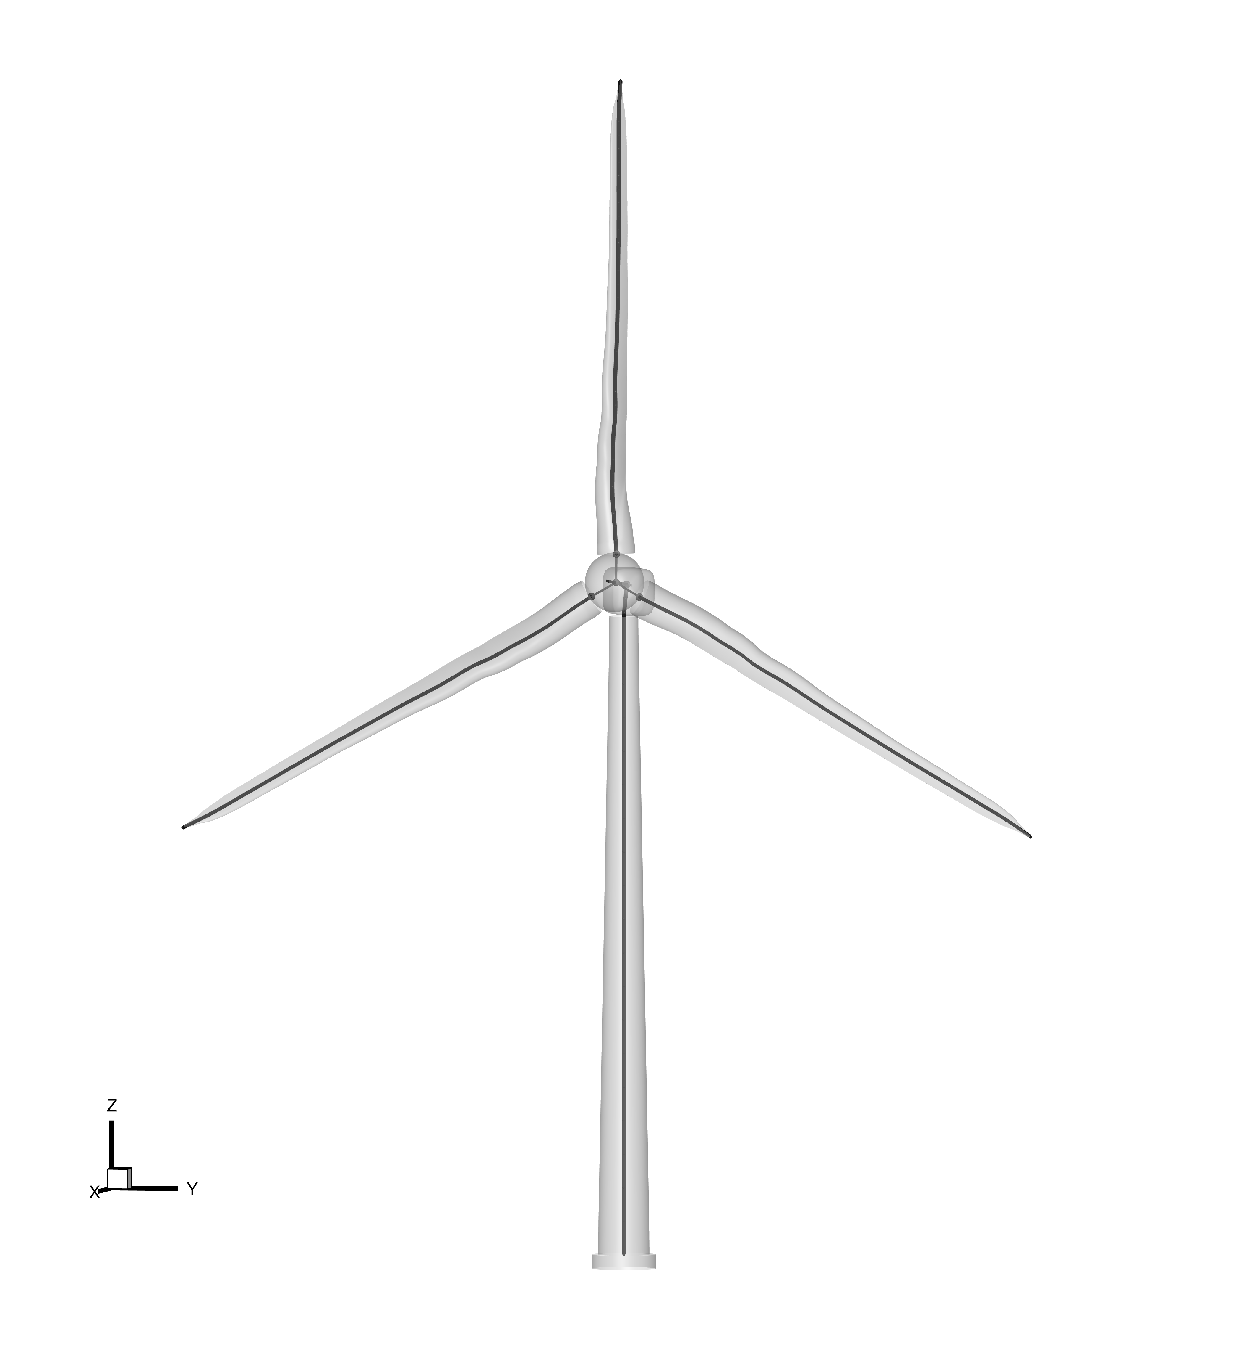
\includegraphics[width=.96\linewidth,height=.43\textheight,keepaspectratio]{figures/tecplot/turbina_3d.pdf}
\caption{Vista tridimensional del aerogenerador y su idealización estructural. Las líneas y los nodos interiores corresponden a las vigas del modelo existente; las envolventes de torre, palas, góndola y cubo facilitan su identificación. Los perfiles de pala y las carcasas son ilustrativos: no proceden de un modelo CAD ni de una discretización de sólidos. Se conservan las coordenadas nodales y la conectividad del modelo.}\label{fig:geometria}\end{figure}

La conversión de los datos conserva 138 nodos y clasifica los 137 elementos originales. Cuatro conectores de penalización se sustituyen por restricciones cinemáticas y por una conexión elástica entre góndola y cubo. Permanecen 133 vigas flexibles: 19 de torre, 35 por pala y nueve transiciones. Las secciones se asignan por estación y los ejes de cada pala se construyen con sus propios puntos auxiliares; no se copia la orientación de una pala a las otras. Esta conversión es distinta del refinamiento espacial posterior, que subdivide los elementos sin modificar sus propiedades por tramos.

Cada nodo tiene tres traslaciones y tres rotaciones, $\bm q_i=[u_i,v_i,w_i,\theta_{xi},\theta_{yi},\theta_{zi}]^\tr$. Los maestros de góndola y cubo son los nodos 129 y 130. Las raíces 21, 57 y 93 se vinculan al cubo mediante brazos rígidos; las puntas son 56, 92 y 128. Se pasa de 828 coordenadas nodales a 810 independientes y, al fijar las seis componentes de la base, a 804 coordenadas de análisis. La eliminación de coordenadas dependientes es exacta; no debe confundirse con el truncamiento modal posterior.

El eje de giro y la velocidad angular se definen por
\begin{equation}
 \bm e_\Omega=\frac{\bm x_{130}-\bm x_{129}}{\|\bm x_{130}-\bm x_{129}\|},\qquad
 \bm\Omega=\Omega\bm e_\Omega,\qquad \Omega=\frac{2\pi}{60}n_{\rm rpm}.
\end{equation}
La velocidad se prescribe, sin una ecuación de control del generador. El giro relativo del tren es una coordenada perturbada distinta del movimiento nominal; su frecuencia depende de la rigidez torsional y no tiene por qué ser cero.

\subsection{Propiedades seccionales e inercias}
Se distinguen los momentos geométricos $I_y,I_z,J_t$ [$\mathrm{m^4}$] de los momentos másicos por unidad de longitud $j_x,j_y,j_z$ [$\mathrm{kg\,m}$]. Para una sección plana en $yz$,
\begin{equation}
 \mu=\int_A\rho\,\dd A,\qquad
 \bm j_C=\int_A\rho\big[(\bm r^\tr\bm r)\I-\bm r\bm r^\tr\big]\dd A,
 \qquad j_x=j_y+j_z.
 \label{eq:inercia}
\end{equation}
La constante torsional $J_t$ no se obtiene de esta identidad. Para la torre se emplean $E=210$ GPa, $\nu=0.3$, $\rho=7850$ kg/m$^3$ y $G=E/[2(1+\nu)]$. Sus propiedades son $EA$, $GA_{sy}$, $GA_{sz}$, $GJ_t$, $EI_y$ y $EI_z$, con áreas efectivas de cortante. La masa e inercia lineales son $\mu=\rho A$ y $\bm j_C=\rho\diag(I_y+I_z,I_y,I_z)$.

Las 35 estaciones de pala proporcionan directamente las seis rigideces generalizadas. Sus columnas de masa se normalizan con un único factor adimensional,
\begin{equation}
 \begin{aligned}
 c_b&=\frac{111484}{\sum_{s=1}^{35}\mathrm{AXIALD}_s(100/35)},\\
 (\mu_s,j_{y,s},j_{z,s})&=c_b(\mathrm{AXIALD}_s,\mathrm{INERT2}_s,\mathrm{INERT3}_s).
 \end{aligned}
 \label{eq:normalizacion}
\end{equation}
Al no disponer de una inercia polar utilizable se adopta $j_x=j_y+j_z$. Los offsets y productos de inercia seccionales se suponen nulos. La masa final se integra sobre las longitudes geométricas reales, lo que explica las pequeñas diferencias entre palas de la Tabla~\ref{tab:masas}.

\begin{table}[htbp]\centering\small
\begin{tabular}{lrrr}\toprule
Componente & Elementos & Longitud [m] & Masa [kg]\\\midrule
Torre &19&135.0000&859784.72\\
Pala 1 &35&100.0820&111605.61\\
Pala 2 &35&100.0821&111608.51\\
Pala 3 &35&100.0899&111623.52\\
Transiciones &9&7.1905&26488.80\\
Góndola &--&--&1184500.00\\
Cubo &--&--&196000.00\\\midrule
Total &133&--&2601611.15\\\bottomrule
\end{tabular}
\caption{Distribución de masa. Las transiciones conservan las propiedades disponibles; no constituyen una caracterización independiente de cojinetes.}\label{tab:masas}
\end{table}

Para góndola y cubo, los tensores centroidales corporales son
\begin{equation}
 \bm J_N^b=\diag(14806000,32672000,32672000),\qquad
 \bm J_H^b=2822400\I\quad[\mathrm{kg\,m^2}].
\end{equation}
La orientación corporal a global, obtenida de la convención ZXZ heredada $(90^\circ,-5^\circ,-90^\circ)$, produce $\bm J_C^g=\bm Q_b\bm J_C^b\bm Q_b^\tr$. Se conservan los productos de inercia generados: para la góndola, $J_{xz}=1.551199\times10^6$ kg m$^2$. Los centros de masa se sitúan en sus maestros por ausencia de offsets disponibles. El centro de masa global resulta $(0.460663,\,2.251\times10^{-6},\,113.886566)$ m.

\section{FORMULACIÓN ENERGÉTICA Y REDUCCIÓN}
\label{sec:formulacion}
\subsection{Elemento de Timoshenko y masa espacial}
En el triedro local del elemento, la deformación generalizada y su energía son
\begin{align}
 \bm\varepsilon&=[u',\ v'-\theta_z,\ w'+\theta_y,\ \theta_x',\ \theta_y',\ \theta_z']^\tr,
 \qquad \bm n=\bm K_s\bm\varepsilon,\\
 U_e&=\tfrac12\int_0^L\bm\varepsilon^\tr\bm K_s\bm\varepsilon\,\dd x,
 \quad \bm K_s=\diag(EA,GA_y,GA_z,GJ_t,EI_y,EI_z).
\end{align}
Se utiliza la interpolación cerrada de dos nodos, que retiene cortante e inercia rotacional. Sus matrices de rigidez e interpolación se desglosan en el Apéndice~\ref{ap:elemento}. Si $\bm r$ es el offset seccional del centro de masa y $\Sx r\bm v=\bm r\times\bm v$, la masa espacial es
\begin{equation}
 \bm M_6=\begin{bmatrix}
 \mu\I&-\mu\Sx r\\ \mu\Sx r&\bm j_C-\mu\Sx r^2
 \end{bmatrix},\qquad
 \bm M_e=\int_0^L\bm N^\tr\bm M_6\bm N\,\dd x.
 \label{eq:masa6}
\end{equation}
El término $-\mu\Sx r^2$ es el traslado de Steiner. La misma expresión, con masa y tensor totales, representa cada cuerpo rígido. La masa consistente y las contribuciones de giro se integran con la misma cinemática y cuatro puntos de Gauss. Los cambios de componentes locales a globales se aplican por congruencia antes del ensamblaje.

\subsection{Equilibrio de operación y tangente elástica}
La precarga se obtiene mediante una energía corrotacional: se actualizan cuerda y marco elemental, se elimina el movimiento rígido y se evalúa $U_e=\tfrac12\bm d_e^\tr\bm K_e\bm d_e$. Se emplean la extensión $L_c-L$ y pequeñas rotaciones deformacionales. El gradiente y la Hessiana de esa misma energía proporcionan $\bm f_{\rm int}$ y $\bm K_{\rm int}$. Las masas e inercias se mantienen en la configuración nominal; por tanto, el modelo combina precarga corrotacional e inercia de referencia, no una linealización inercial exacta sobre toda la configuración deformada.

La conexión góndola--cubo conserva el brazo $\bm d=\bm x_H-\bm x_N$. Su deformación es $\bm\Delta=[(\bm u_H-\bm u_N+\Sx d\bm\theta_N)^\tr,(\bm\theta_H-\bm\theta_N)^\tr]^\tr=\bm B_d\bm q_f$, y su rigidez es $\bm K_d=\bm B_d^\tr\bm k_d\bm B_d$. Así, una rotación rígida compatible no genera deformación artificial en la conexión.

En el azimut de referencia, el equilibrio se expresa como
\begin{equation}
 \bm T_0^\tr\big[\bm f_{\rm int}(\bm q_0)-\bm f_g-
 \bm f_\Omega(\bm q_0)-\bm f_a(\bm q_0,\bm0)-\bm f_{\rm ap}\big]=\bm0,
 \qquad \bm q_0=\bm T_0\bm q_{r0}.
 \label{eq:equilibrio}
\end{equation}
La fuerza interna incluye tren y base; las reacciones esenciales desaparecen por proyección. Newton utiliza la derivada del residual, con búsqueda de paso y continuación en velocidad. Se define $\bm K_{\rm prestress}=\bm K_{\rm int}(\bm q_0)-\bm K_{\rm el}$ para separar la modificación elástica por precarga. No se suma otra rigidez geométrica si esa contribución ya está contenida en la Hessiana.

\subsection{Derivación conjunta de giroscopía y centrifugación}
\label{sec:gyro}
Sea $\bm W=\Sx\Omega$, $\dot{\bm R}_0=\bm R_0\bm W$ y $\bm E(\bm\theta)=\exp(\Sx\theta)$. Para una sección cuyo punto de referencia está a $\bm a$ del eje y cuyo centro de masa tiene offset $\bm r$,
\begin{equation}
 \bm x_C=\bm R_0(\bm a+\bm u+\bm E\bm r),\qquad
 \bm\omega_C=\bm\Omega+\bm J_\ell(\bm\theta)\dot{\bm\theta},
\end{equation}
donde $\bm J_\ell$ es el Jacobiano izquierdo de las rotaciones. Expresando las velocidades en el marco nominal,
\begin{align}
 \bm v_C&=\bm W(\bm a+\bm u+\bm E\bm r)+\dot{\bm u}
       +[\bm J_\ell\dot{\bm\theta}]_\times\bm E\bm r,\\
 \mathcal T&=\tfrac12\mu\bm v_C^\tr\bm v_C
 +\tfrac12\bm\omega_C^\tr\bm E\bm j_C\bm E^\tr\bm\omega_C.
 \label{eq:energiaexacta}
\end{align}
La rotación del tensor $\bm E\bm j_C\bm E^\tr$ es necesaria cuando la inercia es anisótropa. Al expandir hasta segundo orden en $\bm\eta=[\bm u^\tr,\bm\theta^\tr]^\tr$ y sus velocidades,
\begin{equation}
 \mathcal T^{(2)}=\tfrac12\dot{\bm\eta}^\tr\bm M_6\dot{\bm\eta}
 +\dot{\bm\eta}^\tr\bm A_6\bm\eta
 +\tfrac12\bm\eta^\tr\bm H_\Omega\bm\eta.
 \label{eq:energia2}
\end{equation}
Las ecuaciones de Lagrange dan $\bm G_{c,6}=\bm A_6-\bm A_6^\tr$, $\bm K_{\Omega,c}=-\bm H_\Omega$ y $\bm f_\Omega(\bm\eta)=\bm f_{\Omega,0}+\bm H_\Omega\bm\eta$. Este procedimiento sigue la sección 4.4 de \citet{meirovitch1997}; las matrices de seis coordenadas son la especialización para la cinemática seccional aquí definida.

Con $\bm B_C=[\I,-\Sx r]$ y $\bm E_\theta=[\bm0,\I]$, el resultado giroscópico es
\begin{equation}
 \boxed{\bm G_{c,6}=2\mu\bm B_C^\tr\bm W\bm B_C+
 \bm E_\theta^\tr(\bm j_C\bm W+\bm W\bm j_C-\Sx{j_C\Omega})\bm E_\theta.}
 \label{eq:G6}
\end{equation}
Su antisimetría se obtiene de la energía, sin imponerla posteriormente. Para giro sobre el eje principal 1, el coeficiente transversal rotacional es $(j_2+j_3-j_1)\Omega$, no simplemente $j_1\Omega$. La fuerza centrífuga y su tangente deben derivarse conjuntamente, ya que modificar solo el término lineal en velocidad no conserva la misma aproximación mecánica. Las matrices expandidas y el caso de giro no principal se presentan en el Apéndice~\ref{ap:gyro}.

\subsection{Transporte inercial y restricciones temporales}
\label{sec:mapas}
Los operadores corrotantes de palas y cubo se transportan a ejes inerciales antes de acoplarlos con torre y góndola. En el instante de referencia puede tomarse coincidente la orientación de ambos marcos, pero no sus derivadas. Con $\bm W_n$ formado por un bloque $\bm W$ para cada traslación y rotación nodal rotante,
\begin{align}
 \dot{\bm M}_I&=\bm W_n\bm M-\bm M\bm W_n,\qquad
 \bm G_I=\bm G_c-\bm M\bm W_n-\bm W_n\bm M,\\
 \bm D_I&=\bm C_I+\bm G_I+\dot{\bm M}_I,\qquad
 \bm K_{\rm transport}=-\bm G_c\bm W_n+\bm M\bm W_n^2,\\
 \bm K_I&=\bm K_{\rm el}+\bm K_{\rm prestress}
 +\bm K_{\Omega,c}+\bm K_{\rm transport}+\bm K_a.
 \label{eq:transport}
\end{align}
Se conservan por separado la giroscopía antisimétrica y la derivada simétrica de masa. Esta última no es disipación material. Para un cuerpo centrado, el bloque rotacional inercial es $\bm G_{I,\theta}=-[\bm J_C\bm\Omega]_\times$; la parte traslacional de Coriolis desaparece en coordenadas inerciales. No hay contradicción con \eqref{eq:G6}: son expresiones del mismo modelo en coordenadas distintas.

La restricción raíz--cubo es temporal porque gira su brazo. Si $\bm r_s(t)$ une cubo y raíz,
\begin{equation}
 \begin{bmatrix}\bm u_s\\\bm\theta_s\end{bmatrix}
 =\begin{bmatrix}\I&-\Sx{r_s(t)}\\\bm0&\I\end{bmatrix}
 \begin{bmatrix}\bm u_H\\\bm\theta_H\end{bmatrix},\qquad
 \dot{\bm r}_s=\bm W\bm r_s,\quad \ddot{\bm r}_s=\bm W^2\bm r_s.
\end{equation}
Al ensamblar restricciones y condiciones esenciales se obtiene $\delta\bm q_f=\bm T(t)\bm q_r$. Los operadores independientes son
\begin{align}
 \bm M_r&=\bm T^\tr\bm M_I\bm T,\\
 \bm D_r&=\bm T^\tr(\bm D_I\bm T+2\bm M_I\dot{\bm T}),\\
 \bm K_r&=\bm T^\tr(\bm K_I\bm T+\bm D_I\dot{\bm T}+\bm M_I\ddot{\bm T}).
 \label{eq:mpc}
\end{align}
Una congruencia estática es suficiente solo si $\dot{\bm T}=\ddot{\bm T}=\bm0$. La recuperación de velocidades y aceleraciones debe utilizar esas mismas derivadas.

Para el análisis modal se introduce, después de la reducción, $\bm q_r=\bm P_{\rm MBC}(t)\bm z$, con $\bm P_{\rm MBC}=\bm H(t)\bm B_{\rm MBC}(t)$. La matriz $\bm H$ expresa las tres palas en marcos homólogos y $\bm B_{\rm MBC}$ contiene las coordenadas colectiva, coseno y seno. Las matrices $\overline{\bm M},\overline{\bm D},\overline{\bm K}$ se obtienen aplicando nuevamente \eqref{eq:mpc}, ahora con $\bm P_{\rm MBC}$. Tanto $\bm H$ como $\bm B_{\rm MBC}$ se derivan; sus expresiones completas figuran en el Apéndice~\ref{ap:mapas}. La secuencia es, por tanto, energía corrotante, transporte inercial, restricción temporal y transformación multiblade.

\subsection{Acciones externas y amortiguamiento}
La gravedad se introduce mediante la masa consistente. Una ley aerodinámica distribuida general se representa por fuerzas $\bm p_a$ y momentos $\bm m_a$ por longitud:
\begin{equation}
 \bm f_{a,e}=\int_0^L\bm N^\tr[\bm p_a^\tr,\bm m_a^\tr]^\tr\dd x,
 \quad \bm K_a=-\frac{\partial\bm f_a}{\partial\bm q},\quad
 \bm C_a=-\frac{\partial\bm f_a}{\partial\dot{\bm q}}.
 \label{eq:viento}
\end{equation}
La dependencia de orientación y velocidad relativa permite representar cargas seguidoras y términos no conservativos. Una fuerza seguidora puede dar $\bm K_a\ne\bm K_a^\tr$; no se fuerza su simetría. La ley se mantiene general, de modo que el mismo modelo de carga suministre las fuerzas del equilibrio y sus derivadas dinámicas.

El amortiguamiento mecánico se define sobre las velocidades de perturbación del marco de ensamblaje. La parte estructural es $\bm C_s=\alpha\bm M+\beta\bm K_{\rm el}$. Los objetivos $\zeta=1\%$ en 0.2 y 2 Hz dan $\alpha=0.02284795$ s$^{-1}$ y $\beta=0.001446863$ s. La relación $\zeta_j=\alpha/(2\omega_j)+\beta\omega_j/2$ se refiere al par de calibración $(\bm K_{\rm el},\bm M)$; el amortiguamiento modal operativo se determina del problema cuadrático. Se añaden, cuando corresponden, las contribuciones de tren, base y aerodinámica.

\subsection{Autovalores, movimiento sísmico y modelos reducidos}
\label{sec:modalrom}
En el rotor detenido, sin precarga ni amortiguamiento, se resuelve $\bm K\bm\phi_i=\omega_i^2\bm M\bm\phi_i$, con $\bm\phi_i^\tr\bm M\bm\phi_j=\delta_{ij}$. Con giro se plantea, en el azimut seleccionado,
\begin{equation}
 (\lambda^2\overline{\bm M}+\lambda\overline{\bm D}+\overline{\bm K})\bm\phi=\bm0.
 \label{eq:qep}
\end{equation}
Se utiliza una linealización generalizada sin invertir explícitamente la masa. Para $\lambda=\sigma+\mathrm i\omega_d$ se distinguen $f_d=|\omega_d|/(2\pi)$, $f_n=|\lambda|/(2\pi)$ y $\zeta=-\sigma/|\lambda|$. Las ramas se emparejan por MAC en una métrica de masa común; en grupos próximos se comparan subespacios, no únicamente vectores individuales.

Para una aceleración de base $\bm a_g(t)$, sea $\bm\Gamma_f$ el campo completo de traslación unitaria en las direcciones excitadas. En las coordenadas independientes, anteriores a MBC,
\begin{equation}
 \bm M_r\ddot{\bm q}_r+\bm D_r\dot{\bm q}_r+\bm K_r\bm q_r
 =-\bm P_g\bm a_g+\delta\bm f_{a,r},\qquad
 \bm P_g=\bm T_0^\tr\bm M_I\bm\Gamma_f.
 \label{eq:sismo}
\end{equation}
La proyección incluye la masa acoplada a los apoyos antes de eliminar las coordenadas prescritas. No equivale, en general, a recortar filas de una influencia cinemática. Se integra mediante Newmark de aceleración media, $\beta_N=1/4$ y $\gamma_N=1/2$ \citep{newmark1971}. Las velocidades y aceleraciones físicas son
\begin{equation}
 \delta\dot{\bm q}_f=\bm T\dot{\bm q}_r+\dot{\bm T}\bm q_r,\qquad
 \delta\ddot{\bm q}_f=\bm T\ddot{\bm q}_r+2\dot{\bm T}\dot{\bm q}_r+\ddot{\bm T}\bm q_r.
 \label{eq:recuperacion}
\end{equation}
Las aceleraciones absolutas de perturbación añaden $\bm\Gamma_f\bm a_g$; no incluyen por esa sola suma la aceleración centrípeta nominal. Las reacciones se obtienen del residual completo y las fuerzas de viga de $\delta\bm n=\bm K_s\bm B\delta\bm q_e$. El Apéndice~\ref{ap:solucion} recoge las expresiones de integración y recuperación.

Para la comparación de orden reducido se usa el estado conservativo estacionario. Con $\bm\Phi_r=[\bm\phi_1,\ldots,\bm\phi_r]$ y $\bm q_r\simeq\bm\Phi_r\bm\eta$, los operadores ROM son
\begin{equation}
 \bm M_\eta=\bm\Phi_r^\tr\bm M_r\bm\Phi_r,\quad
 \bm D_\eta=\bm\Phi_r^\tr\bm D_r\bm\Phi_r,\quad
 \bm K_\eta=\bm\Phi_r^\tr\bm K_r\bm\Phi_r,\quad
 \bm P_\eta=\bm\Phi_r^\tr\bm P_g.
 \label{eq:rom}
\end{equation}
La normalización da $\bm M_\eta=\I_r$. Las frecuencias retenidas coinciden por construcción con las del MHT; la medida relevante de reducción es el error de respuesta forzada y de reacción, no esa identidad modal.

\section{DISEÑO DE LOS CASOS Y MÉTRICAS}
\label{sec:casos}
Se mantienen la geometría, las masas y una conexión de referencia con rigideces traslacionales de $10^9$ N/m y rotacionales de $10^{10}$ N m/rad, sin amortiguamiento adicional del tren. Son parámetros numéricos del estudio, no valores identificados de un generador. La Tabla~\ref{tab:campanas} separa los casos para evitar atribuir a una condición resultados calculados en otra.

\begin{table}[htbp]\centering\small
\begin{tabularx}{\textwidth}{lXXX}\toprule
 & Discretización & Operación & Reducción modal\\\midrule
Estado &0 rpm, sin gravedad &0--12 rpm, gravedad y precarga &0 rpm, sin gravedad\\
Modelo &MHT y variantes de viga &MHT con operadores corregidos &MHT y ROM12--ROM192\\
Base &Libre o fija, según caso &Fija &Fija\\
Excitación &Libre o fuerza de punta &Base sintética, 1 s &Base sintética, 8 s\\
Objetivo &Núcleo, malla y teoría &Equilibrio, Campbell y respuesta local &Error por truncamiento y costo\\\bottomrule
\end{tabularx}
\caption{Condiciones de comparación. En los casos numéricos se toma $\delta\bm f_a=\bm0$ y $\bm K_a=\bm C_a=\bm0$ para aislar la dinámica estructural. La ley general de viento permanece definida por \eqref{eq:viento}.}\label{tab:campanas}
\end{table}

La excitación común procede de una función analítica de desplazamiento,
\begin{equation}
 u_{g,j}=A_j\sin^3(2\pi f_jt),\qquad
 a_{g,j}=\frac{A_j(2\pi f_j)^2}{4}
 [-3\sin(2\pi f_jt)+9\sin(6\pi f_jt)],
 \label{eq:entrada}
\end{equation}
con $(A_x,A_y)=(0.003,0.0018)$ m y $(f_x,f_y)=(0.65,0.90)$ Hz. Las señales inician con desplazamiento, velocidad y aceleración nulos, y contienen componentes de 0.65, 0.90, 1.95 y 2.70 Hz. Su condición sintética permite controlar la comparación; no representan un sismo normativo ni un registro de sitio. El caso operativo usa 1 s y pasos de 0.02 a 0.00125 s; la comparación ROM usa 8 s y $\Delta t=0.0025$ s, con un cálculo adicional a 0.00125 s.

Para frecuencias positivas y una salida escalar $y(t)$, se definen
\begin{align}
 e_{f,i}&=100\frac{|f_i-f_i^{\rm ref}|}{f_i^{\rm ref}},\\
 e_H(y)&=100\sqrt{\frac{\int_0^{t_f}(y-y^{\rm ref})^2\dd t}
 {\int_0^{t_f}(y^{\rm ref})^2\dd t}},\qquad
 e_P(y)=100\frac{|\max|y|-\max|y^{\rm ref}||}{\max|y^{\rm ref}|}.
 \label{eq:errores}
\end{align}
Las integrales se evalúan por trapecios. $e_H$ incluye diferencias de amplitud y fase y puede superar el 100\%; $e_P$ no informa sobre la forma temporal. Se adopta 1\% como umbral comparativo de suficiencia ROM, no como límite reglamentario. Una comparación entre implementaciones se denomina \emph{cambio relativo}, no error frente a una solución física verdadera. Para los ceros rígidos se utilizan residuos adimensionales y rango--nulidad, puesto que dividir por una frecuencia nula carece de sentido.

\section{DISCRETIZACIÓN, MODOS RÍGIDOS Y EFECTO DE LA TEORÍA}
\label{sec:discretizacion}
\subsection{Núcleo rígido y precisión numérica}
Un elemento libre de 12 coordenadas posee seis movimientos rígidos. Para posiciones nodales $\bm x_I,\bm x_J$, la base
\begin{equation}
 \bm Q_R=\begin{bmatrix}
 \I&-\Sx{x_I}\\\bm0&\I\\\I&-\Sx{x_J}\\\bm0&\I
 \end{bmatrix}
 \label{eq:rigidos}
\end{equation}
genera traslaciones y giros infinitesimales que satisfacen $\bm B\bm Q_R=\bm0$. Por tanto, $\bm K\bm Q_R=\bm0$. Con rigideces seccionales positivas, las seis direcciones deformacionales tienen energía positiva; la nulidad es seis y el rango es seis. La positividad de la masa permite distinguir este núcleo físico de una coordenada sin inercia.

En el caso primitivo, de longitud 5 m, se obtienen seis frecuencias deformacionales: 248.467, 289.364, 783.567, 933.509, 954.930 y 1010.603 Hz. El residual $\|\bm K\bm Q_R\|/(\|\bm K\|\|\bm Q_R\|)$ es $2.691\times10^{-18}$. La comprobación se extiende a los 133 elementos y al ensamblaje conectado libre, que conserva seis movimientos rígidos globales. Al fijar la base desaparecen esos seis movimientos y la primera frecuencia estacionaria sin precarga es 0.1677683 Hz.

La frecuencia calculada no debe confundirse con el residual del núcleo. Si $\lambda_K=\omega^2$ presenta una perturbación de redondeo del orden de $\epsilon\lambda_{\rm escala}$, entonces
\begin{equation}
 |f_{\rm num}|\sim\frac{\sqrt{\epsilon\lambda_{\rm escala}}}{2\pi}.
\end{equation}
Por eso un núcleo identificado con residuos de orden $10^{-18}$ puede mostrar frecuencias crudas de orden $10^{-5}$ Hz en un problema elemental de altas frecuencias. Exigir $10^{-15}$ Hz en doble precisión no es un criterio universal. La Figura~\ref{fig:rigidosmalla} presenta la separación espectral en una rigidez equilibrada: los seis valores singulares menores quedan a nivel de redondeo y el séptimo pertenece inequívocamente al subespacio flexible. No se sustituyen los autovalores crudos por ceros para demostrar esa propiedad.

\subsection{Refinamiento del aerogenerador y subsistemas}
Cada elemento original se subdivide en $s=1,2,4,8$ segmentos colineales con sección y orientación constantes. Se conservan los nodos originales, cuerpos, conexiones y masa total. La referencia es la malla de 1064 elementos, no una solución analítica.
\begin{table}[htbp]\centering\small
\begin{tabular}{rrrrrr}\toprule
$s$&Nodos&Elementos&GDL&$f_1$ [Hz]&$\max_{i\le12}e_{f,i}$ [\%]\\\midrule
1&138&133&804&0.1677683144&0.00934542\\
2&271&266&1602&0.1677682857&0.00218987\\
4&537&532&3198&0.1677682786&0.00043620\\
8&1069&1064&6390&0.1677682768&Referencia\\\bottomrule
\end{tabular}
\caption{Convergencia espacial del MHT detenido y sin precarga. La masa permanece en $2601611.15$ kg.}\label{tab:malla}
\end{table}
La malla inicial difiere menos de 0.00935\% en las primeras doce frecuencias; la duodécima cambia de 1.601265 a 1.601115 Hz entre las mallas extremas. Esta estabilidad espacial respalda el intervalo modal examinado, pero no establece la convergencia de los 192 modos utilizados en la reducción de mayor orden.
\begin{figure}[htbp]
\centering
\begin{minipage}{0.96\linewidth}\centering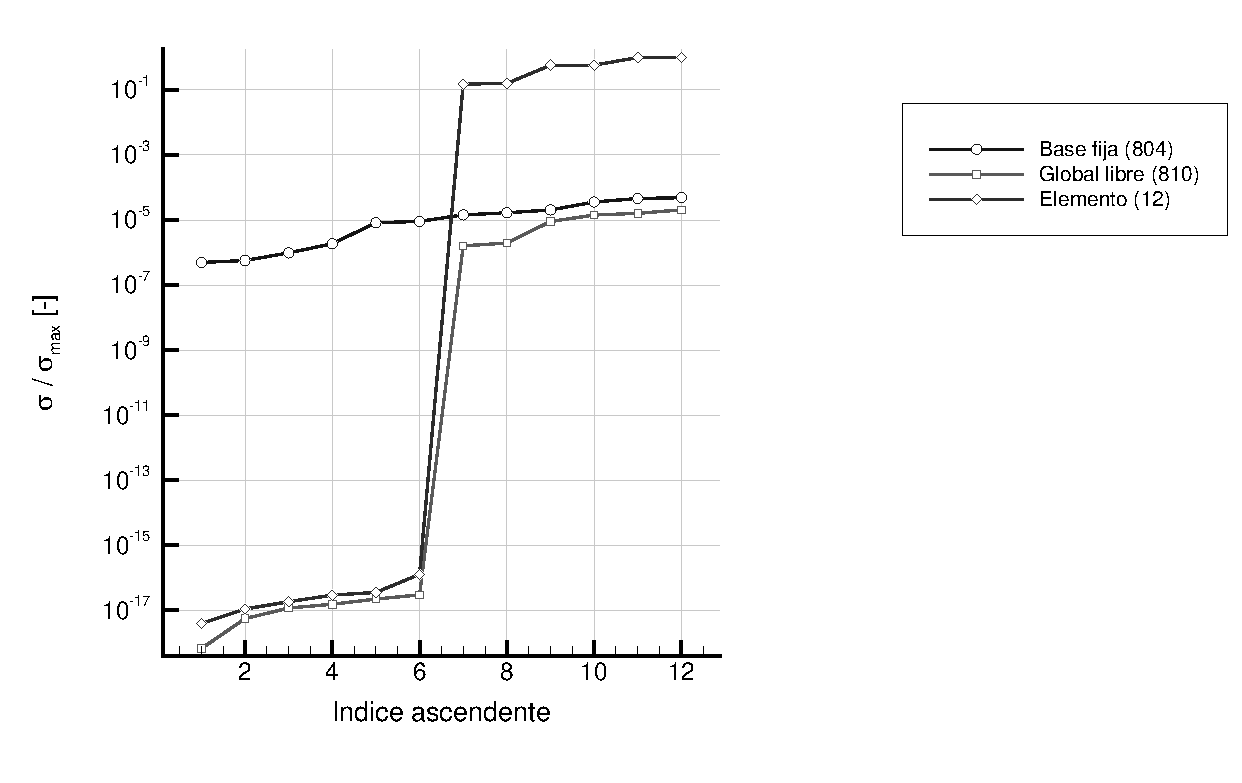
\includegraphics[width=\linewidth]{figures/tecplot/nucleo_rigido.pdf}\end{minipage}
\par\medskip
\begin{minipage}{0.96\linewidth}\centering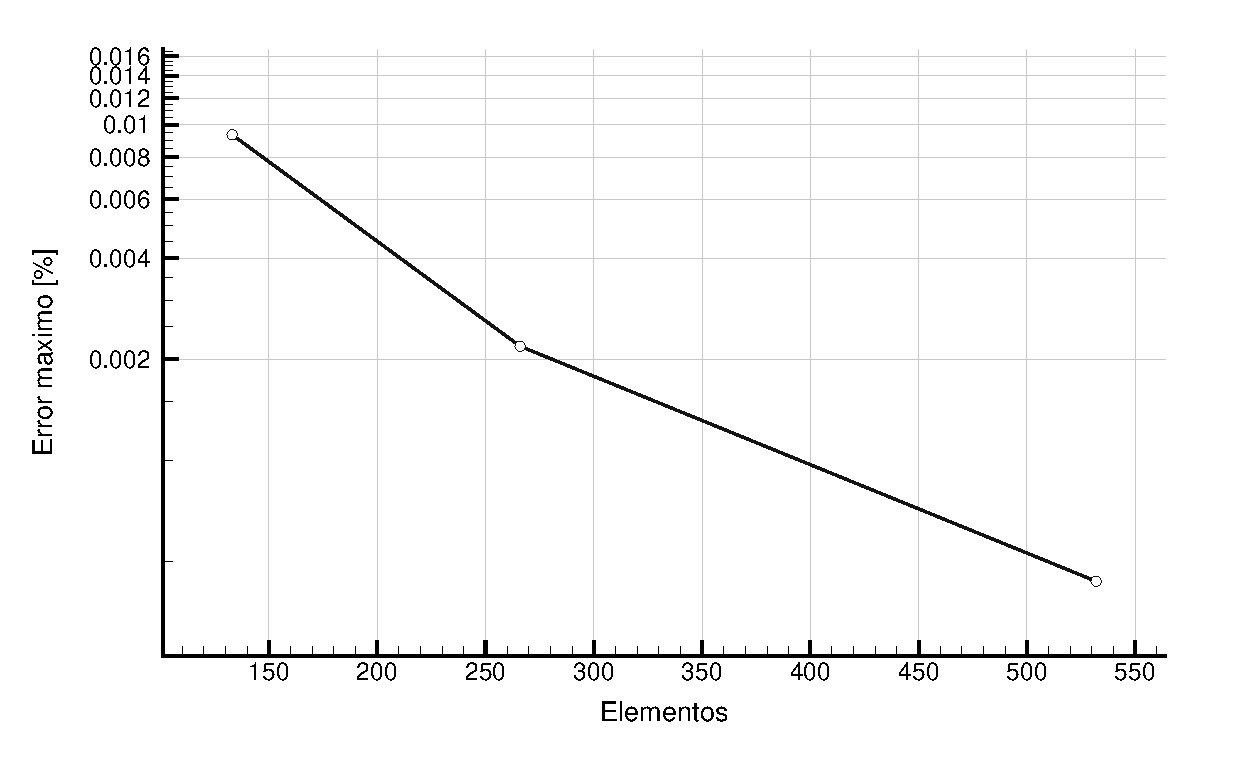
\includegraphics[width=\linewidth]{figures/tecplot/refinamiento.pdf}\end{minipage}
\caption{(a) Valores singulares ascendentes de la rigidez equilibrada $\widehat{\bm K}=\bm S\bm K\bm S$, $\bm S=\diag(K_{ii}^{-1/2})$: seis direcciones rígidas y separación respecto de la séptima. (b) Error máximo de las primeras doce frecuencias respecto de 1064 elementos. El cero de la referencia se conserva en los datos y se omite en la escala logarítmica vertical.}\label{fig:rigidosmalla}\end{figure}

Como comprobación de consistencia de los componentes, las primeras frecuencias en voladizo son 0.7196683 Hz para la torre y 0.4194612, 0.4194880 y 0.4194551 Hz para las tres palas. La máxima dispersión relativa de las frecuencias homólogas de pala es 0.01674\%, coherente con las pequeñas diferencias de geometría y masa. En una viga uniforme auxiliar de 12 m con integración selectiva, 64 elementos dan errores de 0.00610\% en flecha y de 0.00364\% y 0.05838\% en sus dos primeras frecuencias. Este último caso caracteriza una interpolación distinta de la cerrada utilizada en el MHT.

La redistribución HRZ conserva la masa total, pero modifica hasta 1.0738\% las ocho frecuencias de torre examinadas, con MAC mínimo 0.911563. Se utiliza, por ello, masa consistente en las comparaciones principales: conservar únicamente la masa total no garantiza conservar la distribución inercial ni las formas modales.

\subsection{Cortante e inercia rotacional}
Para separar teoría y discretización se comparan voladizos uniformes de 5 m con sección cuadrada de lado 0.5 y 0.05 m, $E=210$ GPa, $\nu=0.3$, $\rho=7850$ kg/m$^3$ y $\kappa=5/6$. Euler--Bernoulli utiliza masa traslacional consistente sin inercia rotacional de flexión y la referencia
\begin{equation}
 f_i^{\rm EB}=\frac{\beta_i^2}{2\pi L^2}\sqrt{\frac{EI}{\rho A}},\qquad
 \beta_i=\{1.875104,4.694091,7.854757,10.995541\}.
\end{equation}
Timoshenko conserva cortante e inercia rotacional y se compara con 512 elementos; el cambio máximo entre 256 y 512 elementos es 0.00118\% en los cuatro modos considerados. Para $L/h=100$, las diferencias entre teorías van de 0.00798 a 0.24486\%; para $L/h=10$, de 0.79293 a 21.20791\%. El refinamiento reduce el error respecto de cada teoría, pero no elimina la diferencia física entre sus hipótesis (Figura~\ref{fig:teorias}).
\begin{figure}[htbp]
\centering
\begin{minipage}{0.96\linewidth}\centering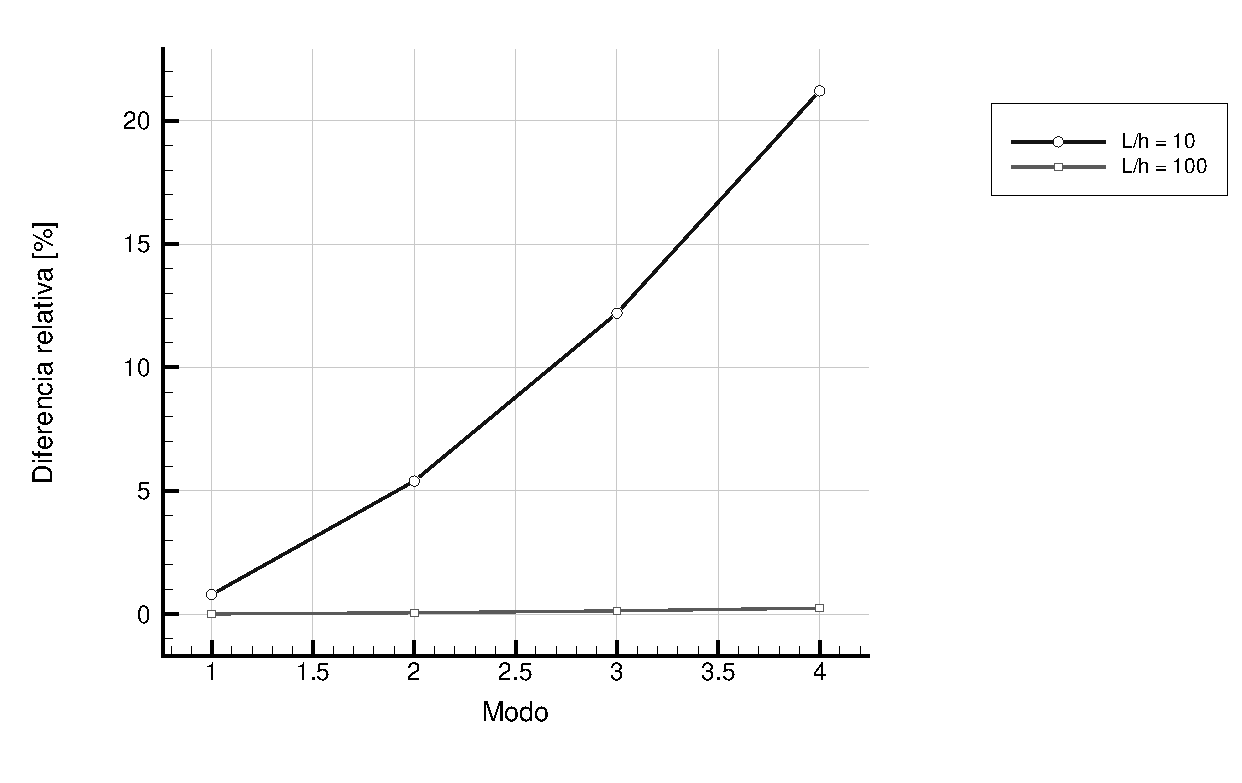
\includegraphics[width=\linewidth]{figures/tecplot/teoria_diferencia.pdf}\end{minipage}
\par\medskip
\begin{minipage}{0.96\linewidth}\centering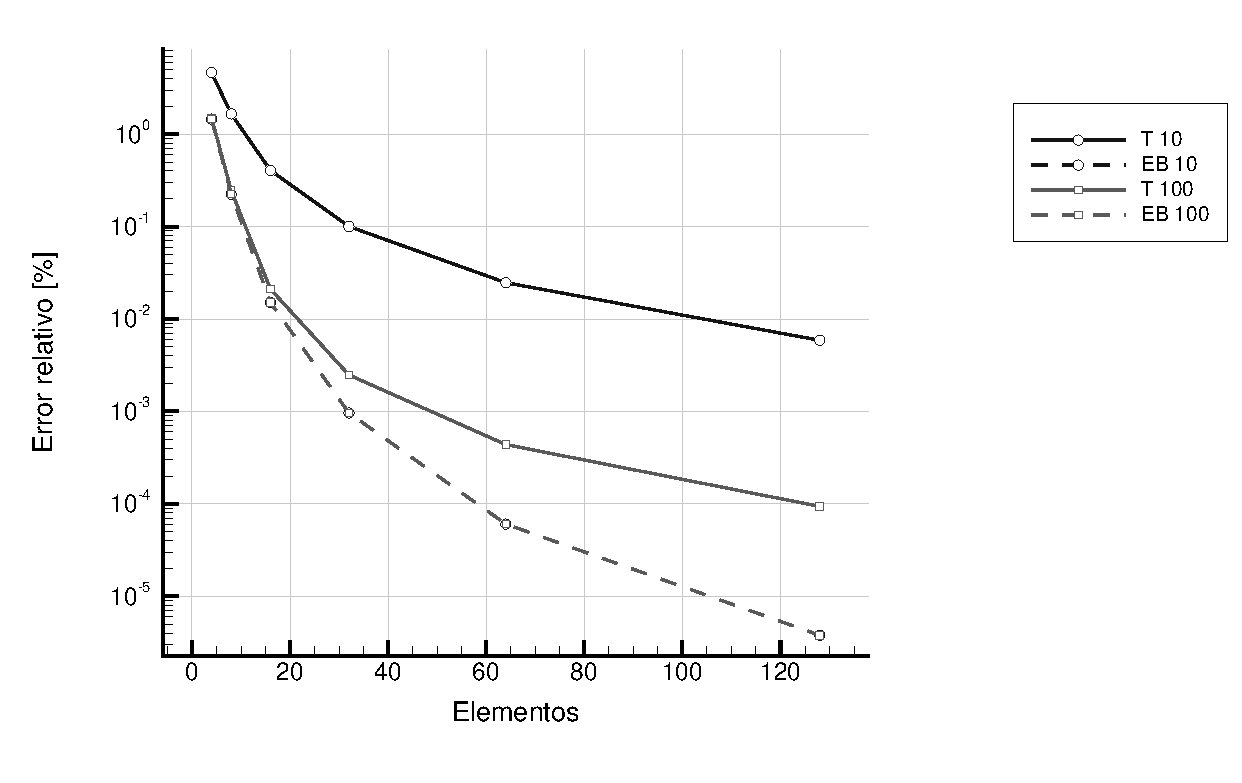
\includegraphics[width=\linewidth]{figures/tecplot/teoria_convergencia.pdf}\end{minipage}
\caption{(a) Diferencia entre Euler--Bernoulli y la referencia Timoshenko para dos esbelteces. (b) Convergencia del cuarto modo de cada teoría respecto de su propia referencia. Las curvas distinguen error de discretización y efecto de la teoría.}\label{fig:teorias}\end{figure}

La misma interpretación se obtiene de las flechas $\delta_{\rm EB}=PL^3/(3EI)$ y $\delta_T=\delta_{\rm EB}+PL/(\kappa GA)$. En el aerogenerador se aísla el cortante imponiendo $GA_y,GA_z\to\infty$, pero conservando las inercias rotacionales: esta variante es de tipo Rayleigh en flexión, no Euler--Bernoulli clásico. Las primeras once frecuencias emparejadas aumentan entre 0.487 y 3.108\%, con MAC mayor o igual a 0.99917. Los modos 12--13 se mezclan; su MAC individual es aproximadamente 0.652, mientras que el MAC subespacial mínimo es 0.99755. La alta coincidencia del subespacio impide interpretar la mezcla de sus vectores como pérdida del modo físico.

% Restored from the persisted operating_results.json; no new solver calls.
\subsection{Equilibrio y espectro del estado operativo}
El barrido corregido contiene nueve velocidades entre 0 y 12 rpm y doce ramas seguidas. Se emplean los resultados almacenados de la revisión energética de septiembre, con gravedad y operadores congelados en el azimut de referencia. Este análisis no representa una órbita periódica ni un problema de Floquet.
La máxima traslación nodal del equilibrio pasa de 1.82421 m a 2.13476 m entre los extremos del barrido. El máximo residuo QEP normalizado almacenado es 2.59222e-16 y el mínimo MAC efectivo es 0.835986. Las multiplicidades se controlan mediante subespacios.
\begin{table}[htbp]\centering\small\caption{Frecuencias amortiguadas de las ramas seguidas en los extremos del barrido corregido.}\begin{tabular}{rrr}\toprule Rama & 0 rpm [Hz] & 12 rpm [Hz]\\\midrule
1 & 0.161234 & 0.154859 \\
2 & 0.163378 & 0.160195 \\
3 & 0.340023 & 0.230491 \\
4 & 0.369133 & 0.379090 \\
5 & 0.378025 & 0.437515 \\
6 & 0.501694 & 0.562695 \\
7 & 0.601075 & 0.612029 \\
8 & 0.636774 & 0.824433 \\
9 & 0.943250 & 0.862845 \\
10 & 0.995952 & 1.229092 \\
11 & 1.152794 & 1.221593 \\
12 & 1.599818 & 1.595477 \\\bottomrule\end{tabular}\end{table}
\begin{figure}[htbp]\centering
\begin{minipage}{0.96\linewidth}\centering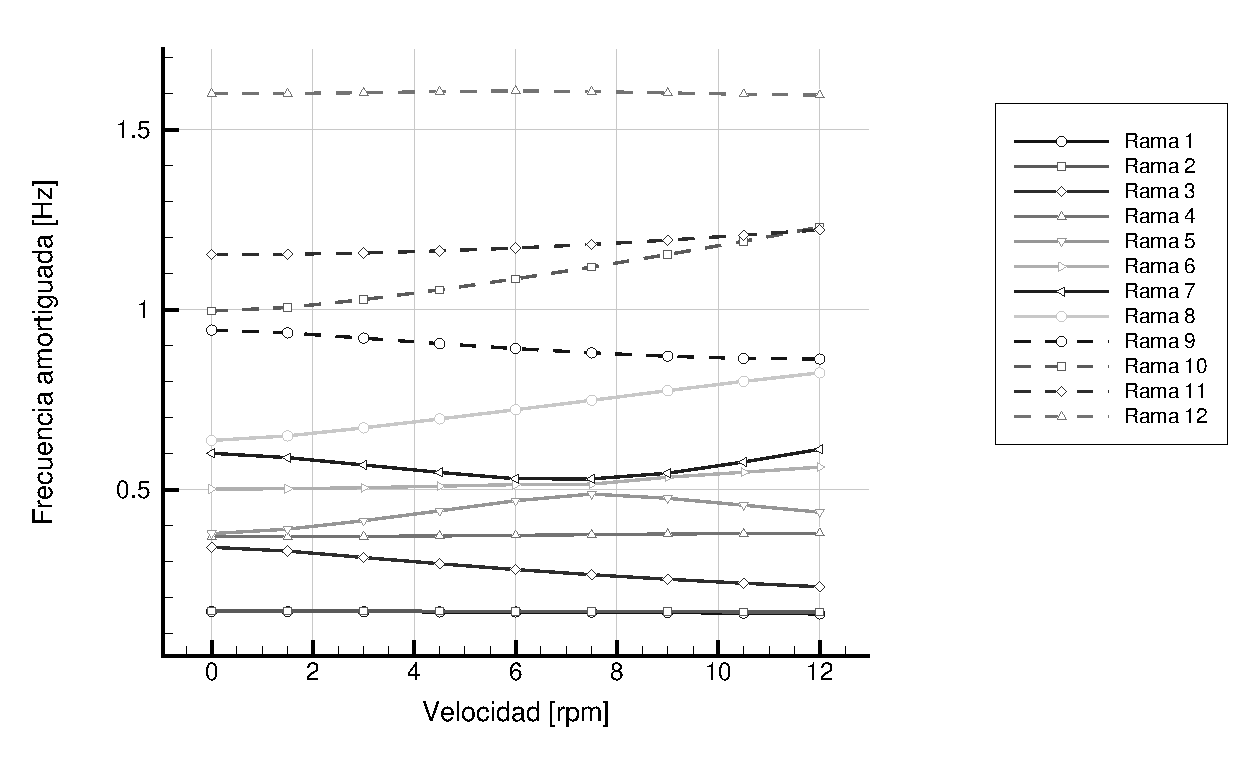
\includegraphics[width=\linewidth]{figures/tecplot/campbell.pdf}\end{minipage}
\par\medskip
\begin{minipage}{0.96\linewidth}\centering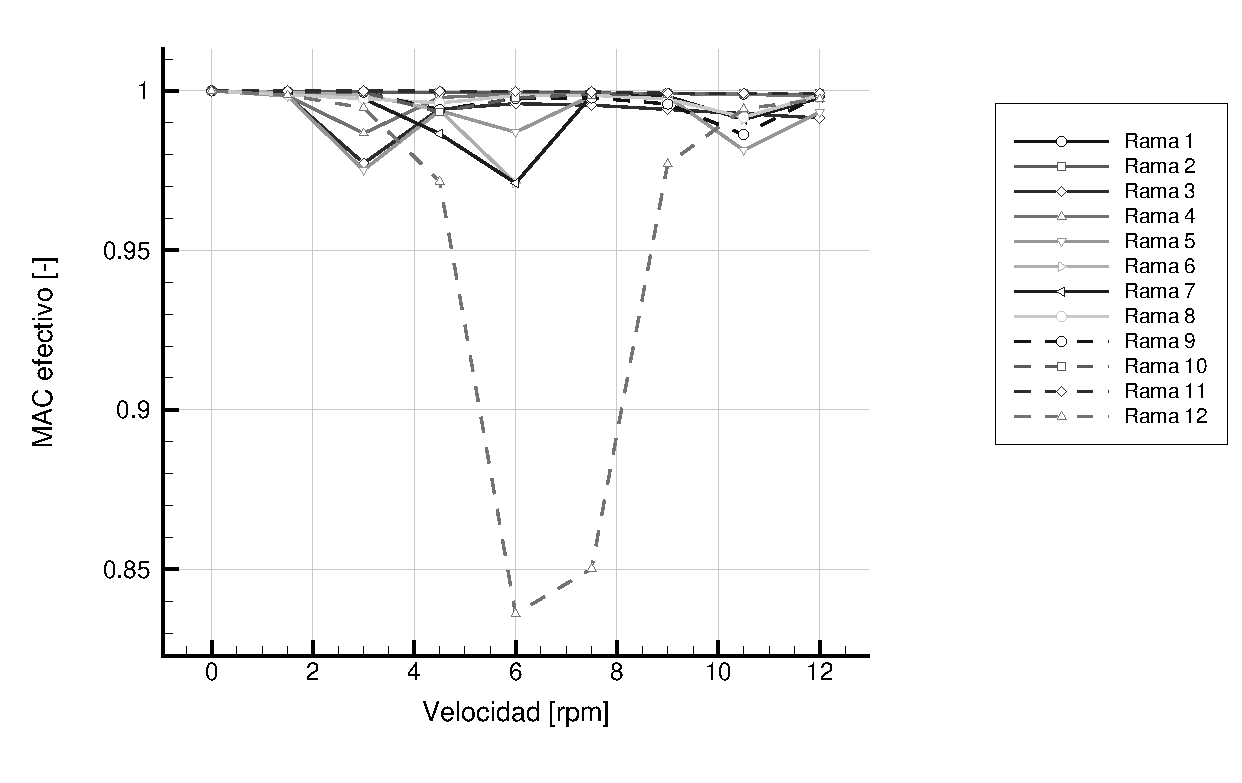
\includegraphics[width=\linewidth]{figures/tecplot/seguimiento_ramas.pdf}\end{minipage}
\caption{(a) Frecuencias amortiguadas del sistema congelado y (b) calidad efectiva del seguimiento por formas. Las líneas unen las velocidades calculadas; no constituyen modos de Floquet.}\label{fig:campbell-tecplot}
\end{figure}
\begin{figure}[htbp]\centering
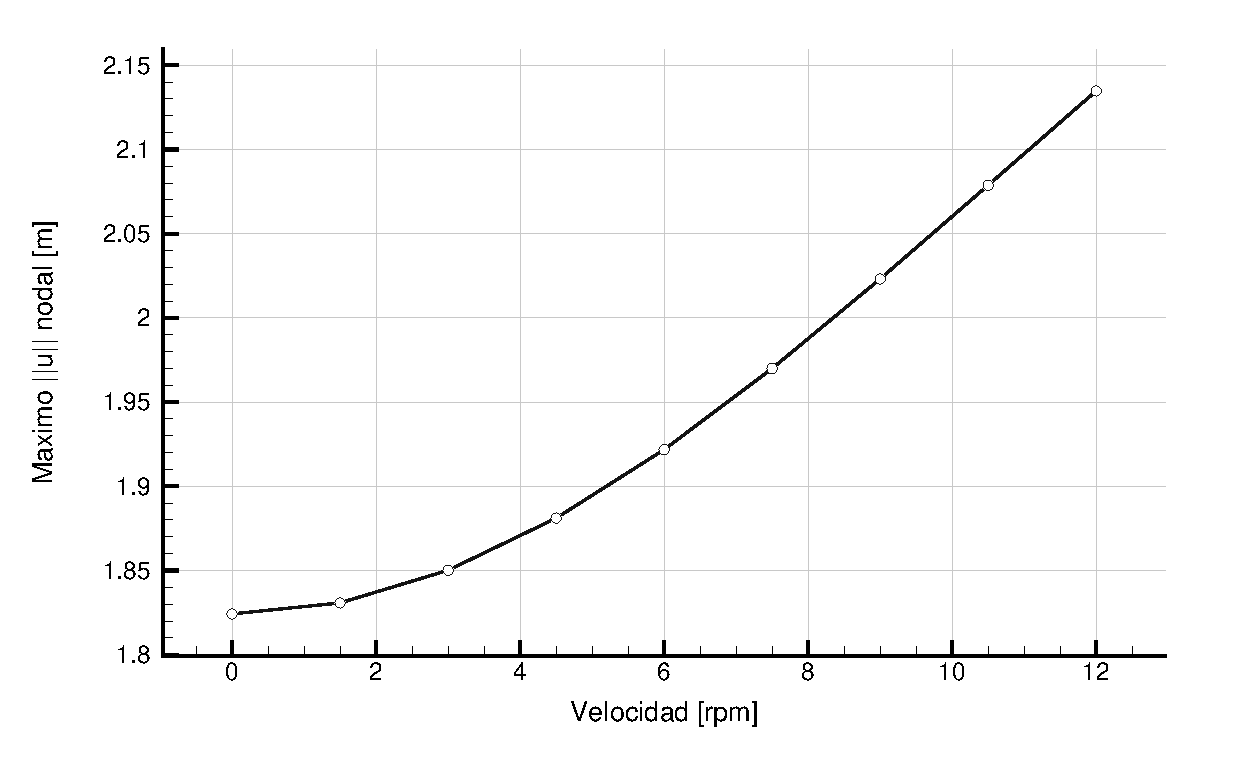
\includegraphics[width=.96\linewidth,height=.40\textheight,keepaspectratio]{figures/tecplot/equilibrio_velocidad.pdf}
\caption{Máxima norma de traslación nodal del equilibrio guardado frente a velocidad. Las líneas unen los estados almacenados.}\label{fig:equilibrio-tecplot}
\end{figure}
\begin{figure}[htbp]\centering
\begin{minipage}{0.96\linewidth}\centering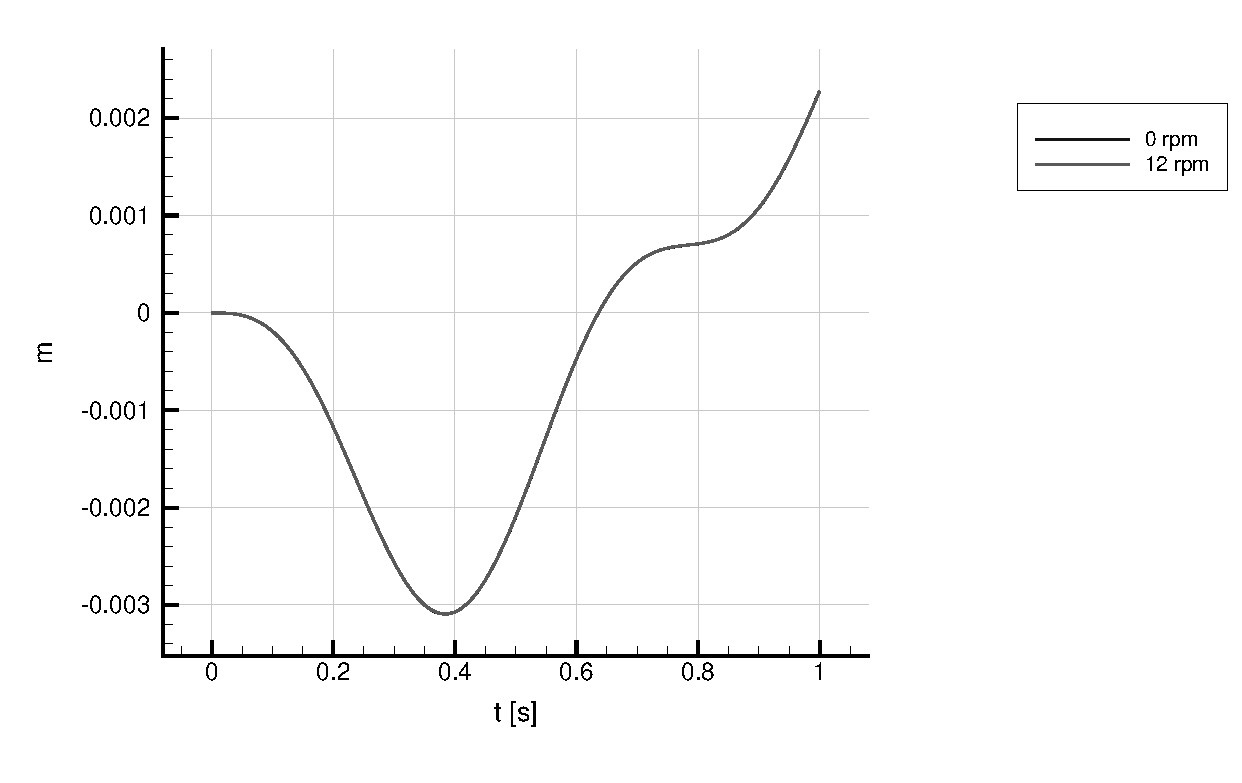
\includegraphics[width=\linewidth]{figures/tecplot/sismo_n129_ux.pdf}\end{minipage}
\par\medskip
\begin{minipage}{0.96\linewidth}\centering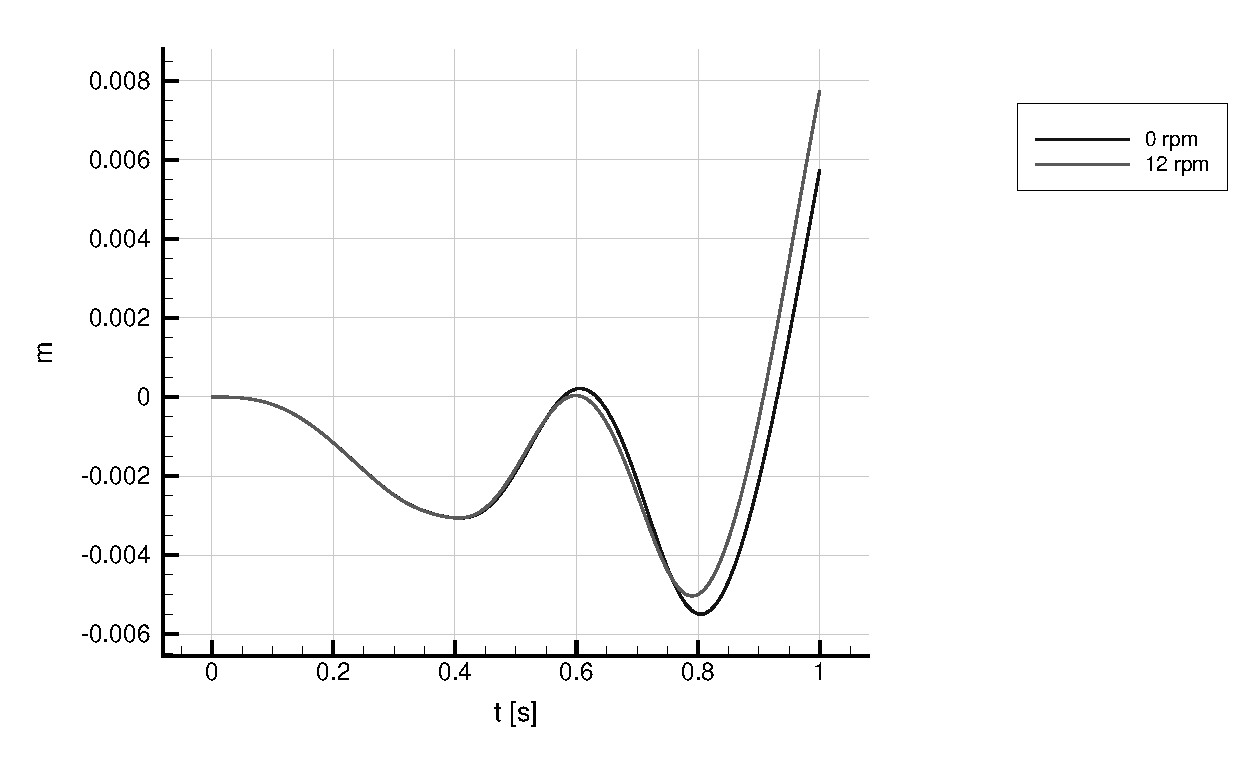
\includegraphics[width=\linewidth]{figures/tecplot/sismo_n56_ux.pdf}\end{minipage}
\caption{Perturbaciones de desplazamiento global X de (a) góndola, nodo 129, y (b) punta de pala 1, nodo 56, en los casos almacenados de 0 y 12 rpm. La ventana y el procesamiento corresponden al benchmark guardado; no se presenta un registro experimental adicional.}\label{fig:sismo-tecplot}
\end{figure}
\begin{figure}[htbp]\centering
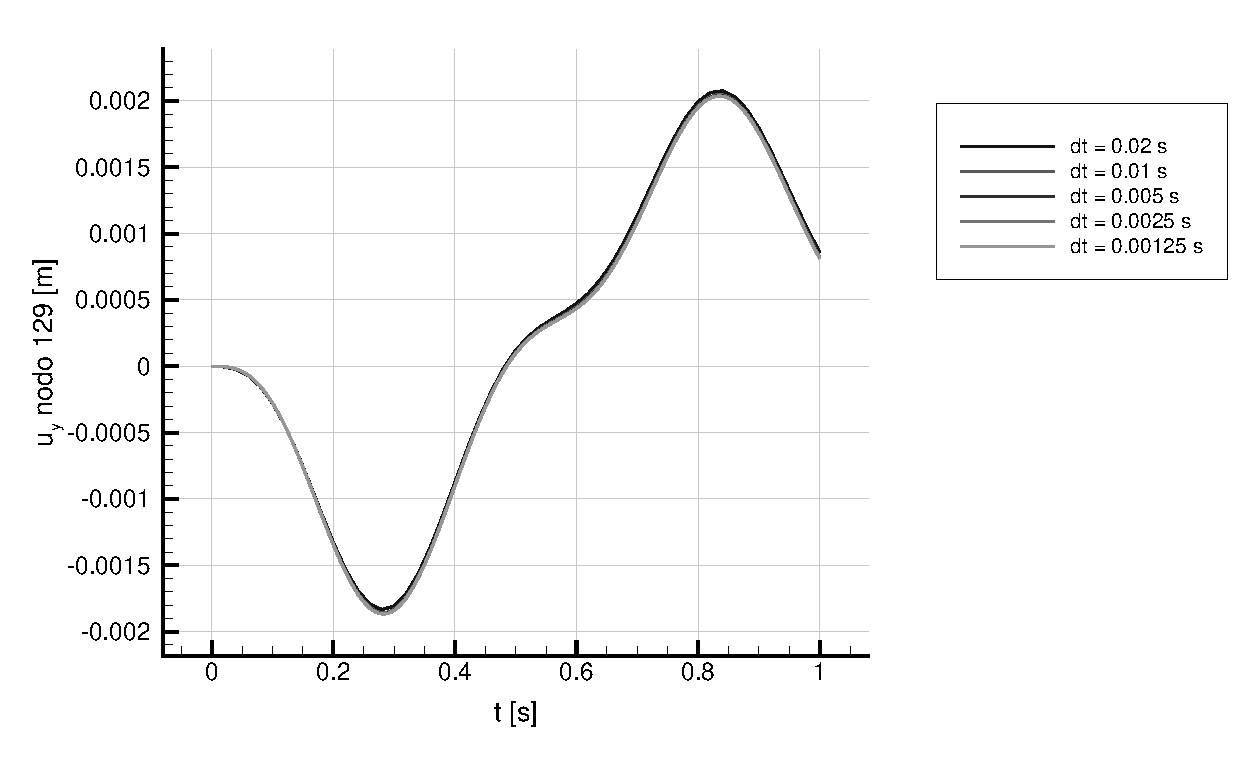
\includegraphics[width=.96\linewidth,height=.40\textheight,keepaspectratio]{figures/tecplot/sismo_convergencia.pdf}
\caption{Comparación temporal del desplazamiento global Y del nodo 129 para los cinco pasos almacenados. Se conserva la ventana de un segundo y la recuperación local de perturbaciones.}\label{fig:sismo-convergencia-tecplot}
\end{figure}
Las matrices y la reconstrucción física corresponden al mismo instante operativo. Las diferencias entre estados de giro incluyen equilibrio, transporte, restricciones temporales y transformación de coordenadas. No se atribuye el cambio de respuesta a un único bloque giroscópico aislado.


\section{PRECISIÓN Y COSTO DE LA REDUCCIÓN MODAL}
\label{sec:resultadosrom}
\subsection{Respuesta forzada y selección de orden}
La comparación utiliza el MHT detenido y sin precarga durante ocho segundos, según la Tabla~\ref{tab:campanas}. Los ROM de 12, 24, 48, 96 y 192 modos tienen frecuencias de corte de 1.6013, 3.3883, 9.1686, 21.9497 y 52.7107 Hz. Todas las bases conservan las mismas propiedades físicas y excitación. Se observan cinco desplazamientos relativos, dos aceleraciones absolutas y el momento basal $M_{b,y}$.

\begin{table}[htbp]\centering\small\setlength{\tabcolsep}{4pt}
\begin{tabular}{lrrrrrr}\toprule
Salida & Pico MHT & ROM12 & ROM24 & ROM48 & ROM96 & ROM192\\\midrule
$u_{129,x}$ [mm]&3.91172&2.4357&0.0470&0.0090&0.0011&0.000025\\
$u_{129,y}$ [mm]&2.48620&6.7463&0.0923&0.0190&0.0025&0.000123\\
$u_{56,x}$ [mm]&14.91031&50.3645&3.1865&0.1932&0.0007&0.000017\\
$u_{92,x}$ [mm]&28.89985&79.9090&2.6288&0.1024&0.0005&0.000009\\
$u_{128,x}$ [mm]&36.61559&90.9597&2.0116&0.0912&0.0003&0.000008\\
$a_{129,x}^{\rm abs}$ [m/s$^2$]&0.02299&63.2904&3.4796&0.4405&0.0422&0.000927\\
$a_{56,x}^{\rm abs}$ [m/s$^2$]&1.08392&111.6740&15.0924&0.8227&0.0023&0.000062\\
$M_{b,y}$ [MN m]&4.60412&98.5584&24.6754&7.1156&1.6071&0.086572\\\bottomrule
\end{tabular}
\caption{Picos de referencia del MHT y errores de historia $e_H$ [\%] de cada ROM, integrados sobre la misma malla temporal. Las unidades de la segunda columna dependen de la salida; las otras cinco columnas son porcentajes.}\label{tab:rom}
\end{table}

El ROM12 describe razonablemente el desplazamiento de góndola, pero su frecuencia de corte queda por debajo de las componentes de entrada de 1.95 y 2.70 Hz. Presenta errores de 50.4--91.0\% en las puntas y de 98.6\% en el momento basal. El ROM24 incorpora ese intervalo y mejora la respuesta, aunque conserva diferencias importantes en aceleraciones y reacciones. La inclusión de las frecuencias de excitación es necesaria en este caso, pero no suficiente para todas las salidas.

Con 48 modos, los máximos errores de historia de desplazamiento y aceleración disminuyen a 0.193 y 0.823\%; el momento basal conserva 7.116\%. Este último baja a 1.607\% con 96 modos y a 0.0866\% con 192. Por tanto, ROM48 satisface el criterio del 1\% para las siete salidas de movimiento, mientras que ROM192 es la primera base estudiada que lo satisface para las ocho salidas. Las historias de la Figura~\ref{fig:romhistorias} muestran por qué una buena coincidencia de desplazamientos no garantiza una reacción precisa.
\begin{figure}[htbp]\centering
\begin{minipage}{0.96\linewidth}\centering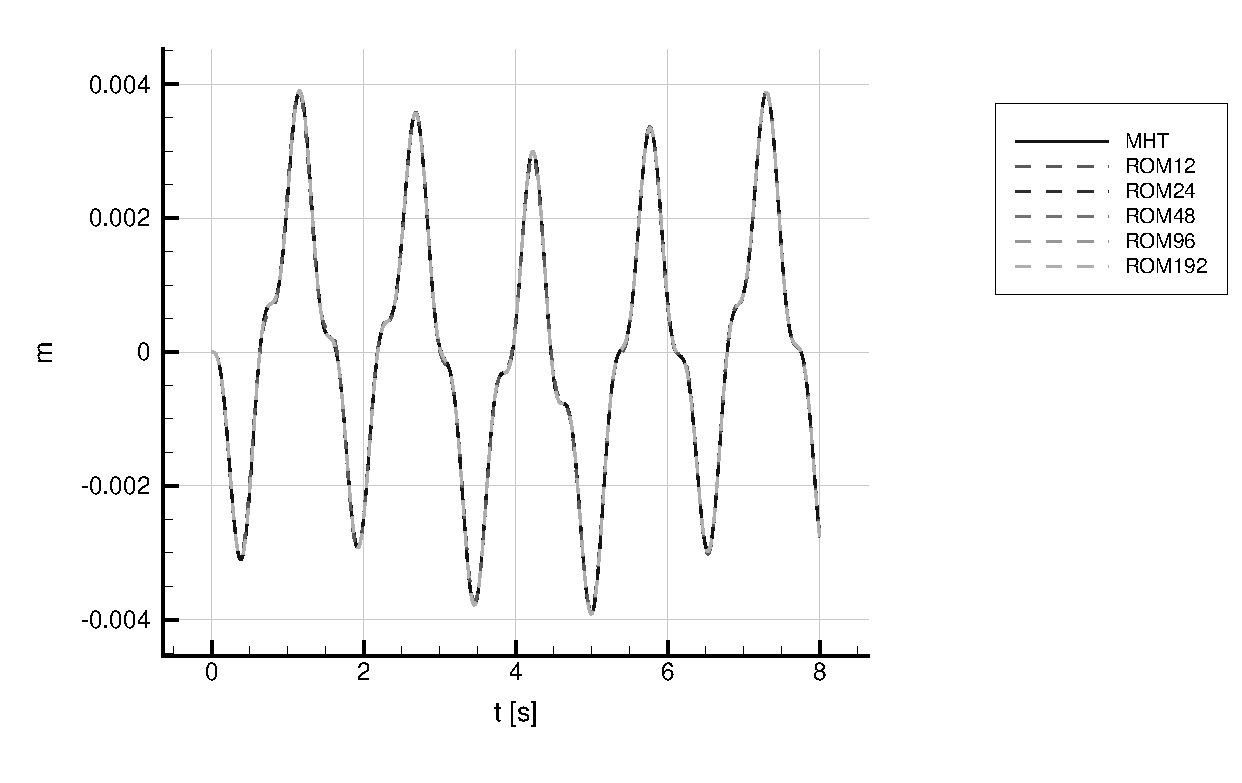
\includegraphics[width=\linewidth]{figures/tecplot/rom_historia_0.pdf}\end{minipage}
\par\medskip
\begin{minipage}{0.96\linewidth}\centering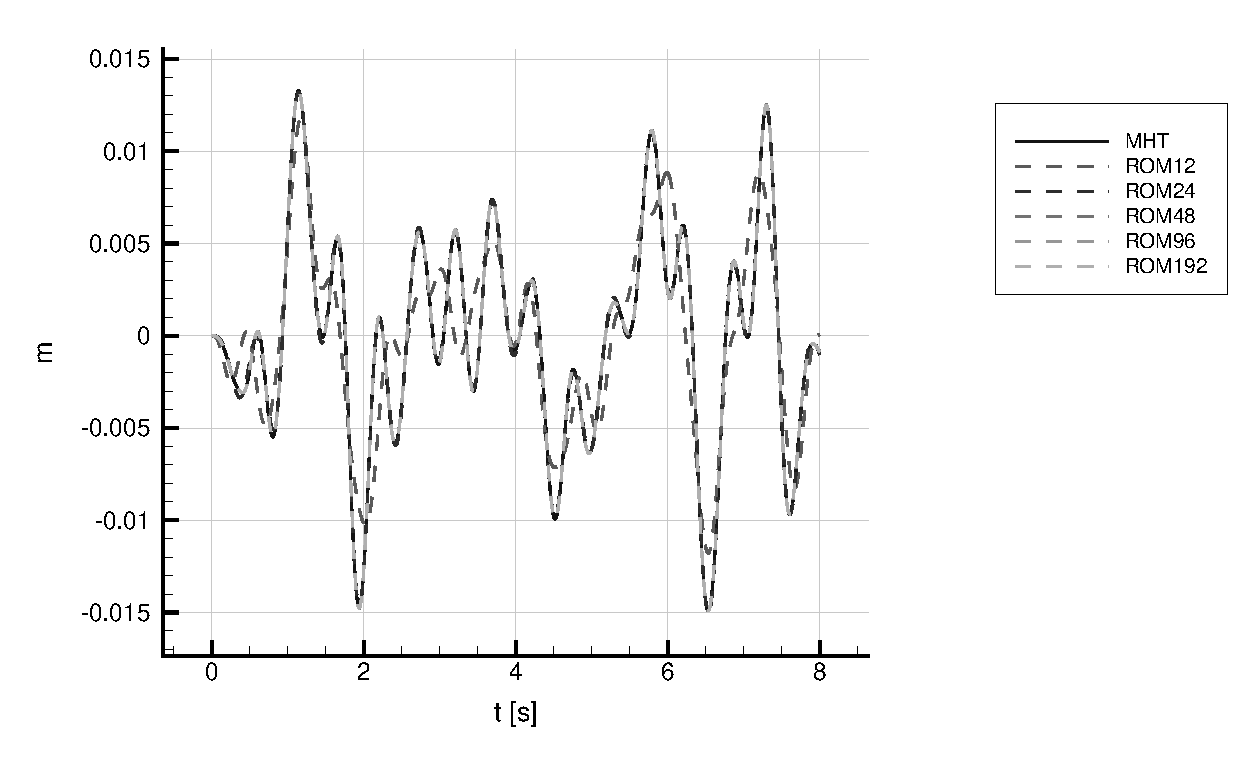
\includegraphics[width=\linewidth]{figures/tecplot/rom_historia_2.pdf}\end{minipage}
\caption{Respuesta estacionaria de ocho segundos: (a) desplazamiento global X de la góndola y (b) de la punta de pala 1. Las curvas son las historias almacenadas del MHT y los ROM seleccionados; su proximidad visual no sustituye los errores de la tabla.}\label{fig:romhistorias}\end{figure}
\begin{figure}[htbp]\centering
\begin{minipage}{0.96\linewidth}\centering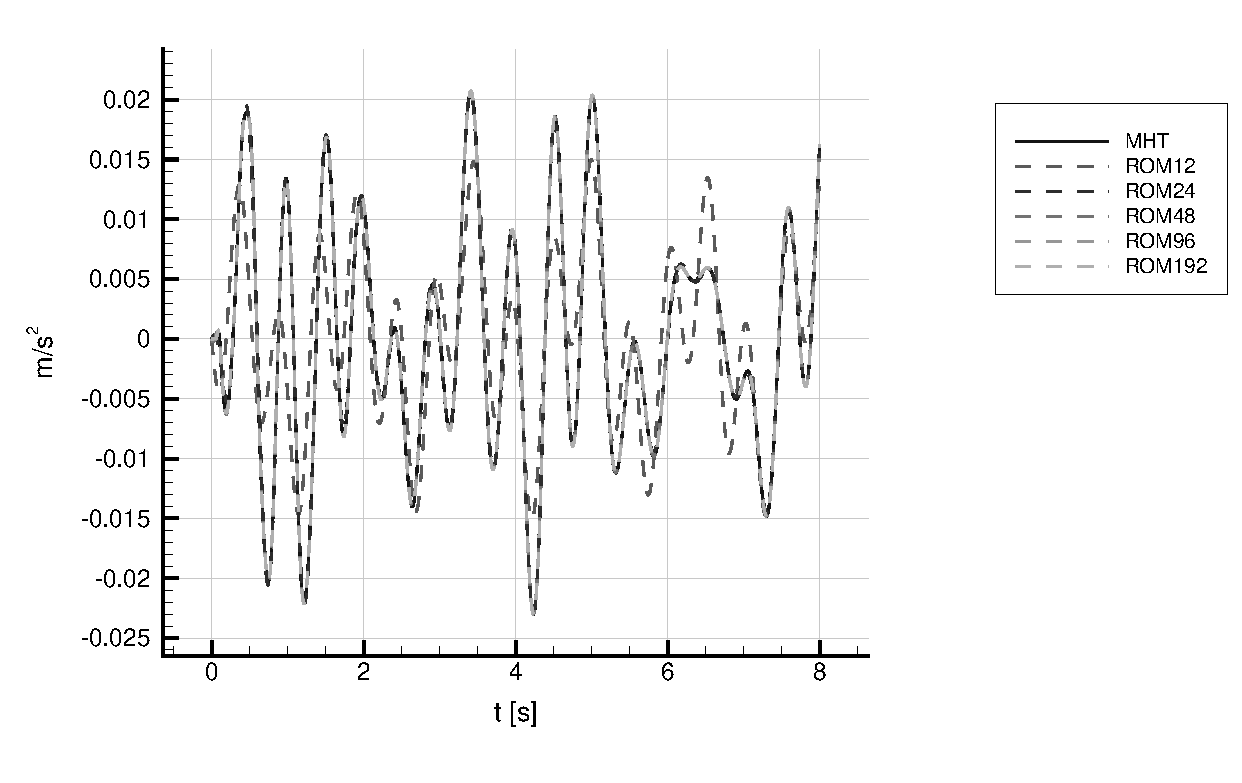
\includegraphics[width=\linewidth]{figures/tecplot/rom_historia_5.pdf}\end{minipage}
\par\medskip
\begin{minipage}{0.96\linewidth}\centering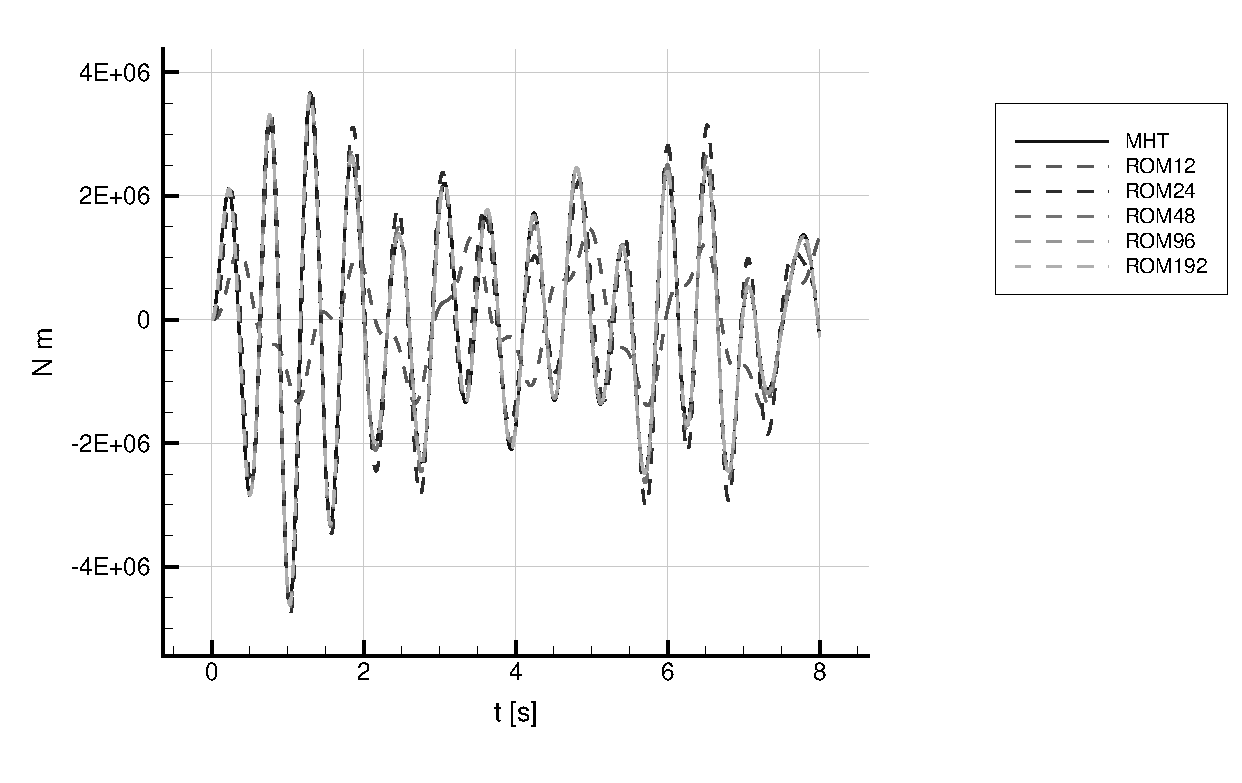
\includegraphics[width=\linewidth]{figures/tecplot/rom_historia_7.pdf}\end{minipage}
\caption{Respuesta estacionaria de ocho segundos: (a) aceleración absoluta global X de la góndola y (b) momento basal global Y. Se conservan las historias almacenadas del MHT y los ROM seleccionados.}\label{fig:romhistorias-continuacion}\end{figure}

La reacción depende de la combinación de inercia, amortiguamiento y rigidez en la coordenada restringida; una forma poco visible en el desplazamiento de un punto puede contribuir al equilibrio del apoyo. Esta dependencia explica que el orden suficiente sea una propiedad de la salida, no un número único del modelo. La Figura~\ref{fig:romcoste} relaciona los errores máximos por tipo de respuesta con la eficiencia computacional.

La fracción de carga inercial capturada se define por
\begin{equation}
 p_{r,j}=100\frac{\sum_{i=1}^{r}(\bm\phi_i^\tr\bm P_{g,j})^2}
 {\bm P_{g,j}^\tr\bm M_r^{-1}\bm P_{g,j}}.
 \label{eq:participacion}
\end{equation}
No es una fracción de la masa total de la turbina, sino de la norma cinética de la carga proyectada admisible. ROM48 captura 93.69\% en $x$ y 94.15\% en $y$; ROM192 alcanza 98.99\% y 99.03\%. La primera base cumple el criterio de movimiento, pero no el de reacción: una participación global elevada tampoco sustituye una comprobación por salida.

\subsection{Costo computacional y error temporal}
Los tiempos se midieron en MATLAB R2026a Update 4, Apple M4 Pro, 24 GiB de memoria y un hilo. Se informa la mediana de tres repeticiones después de un calentamiento, alternando el orden de ejecución. Se separan construcción de base, proyección e integración; esta última incluye los arreglos de respuesta y la evaluación energética del integrador, pero no el ensamblaje común, la recuperación posterior ni la exportación.

\begin{table}[htbp]\centering\small
\begin{tabular}{rrrrrrr}\toprule
GDL & Base [s] & Proy. [s] & Integr. [s] & $S_{\rm int}$ & $S_{\rm caso}$ & Almac. [kB]\\\midrule
804 &--&--&0.459749&1.00&1.00&616.248\\
12 &0.005362&0.000559&0.010126&45.40&28.65&80.640\\
24 &0.003808&0.000729&0.011833&38.85&28.08&168.192\\
48 &0.006835&0.001126&0.027394&16.78&13.00&364.032\\
96 &0.014900&0.002192&0.051313&8.96&6.72&838.656\\
192 &0.049114&0.004009&0.131726&3.49&2.49&2119.680\\\bottomrule
\end{tabular}
\caption{Costo de la campaña estacionaria. $S_{\rm int}=t_{\rm MHT,int}/t_{\rm ROM,int}$ y $S_{\rm caso}=t_{\rm MHT,int}/(t_{\rm base}+t_{\rm proy}+t_{\rm ROM,int})$. El almacenamiento incluye operadores y base, con 1 kB = 1000 bytes; no es memoria pico.}\label{tab:costos}
\end{table}

ROM48 acelera la integración 16.78 veces; al incluir una base nueva y su proyección, la relación es 13.00. Para satisfacer también la reacción basal se requieren 192 modos, con relaciones de 3.49 y 2.49. El ahorro depende, por tanto, de la precisión exigida y de si la base se reutiliza. Además, los operadores densos y la base del ROM192 ocupan 2120 kB, frente a 616 kB del MHT disperso: reducir coordenadas no asegura reducir el almacenamiento matricial.
\begin{figure}[htbp]\centering
\begin{minipage}{0.96\linewidth}\centering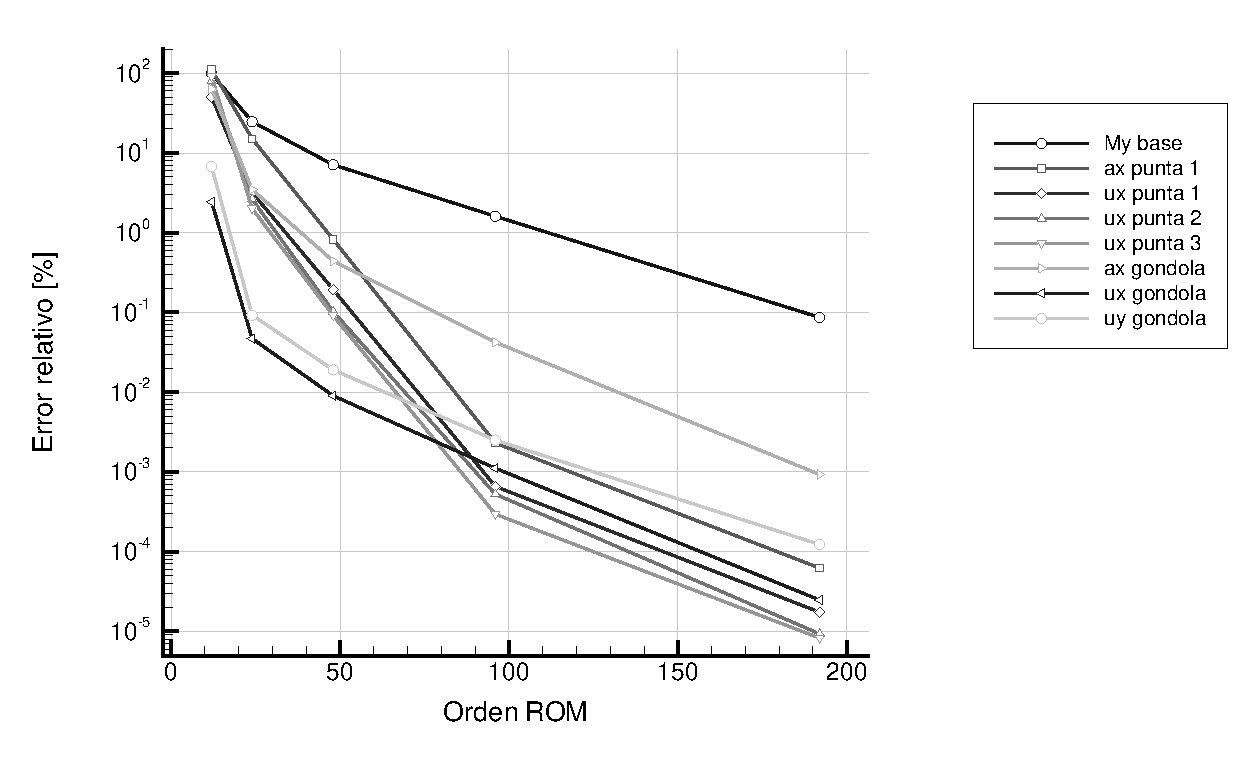
\includegraphics[width=\linewidth]{figures/tecplot/rom_error.pdf}\end{minipage}
\par\medskip
\begin{minipage}{0.96\linewidth}\centering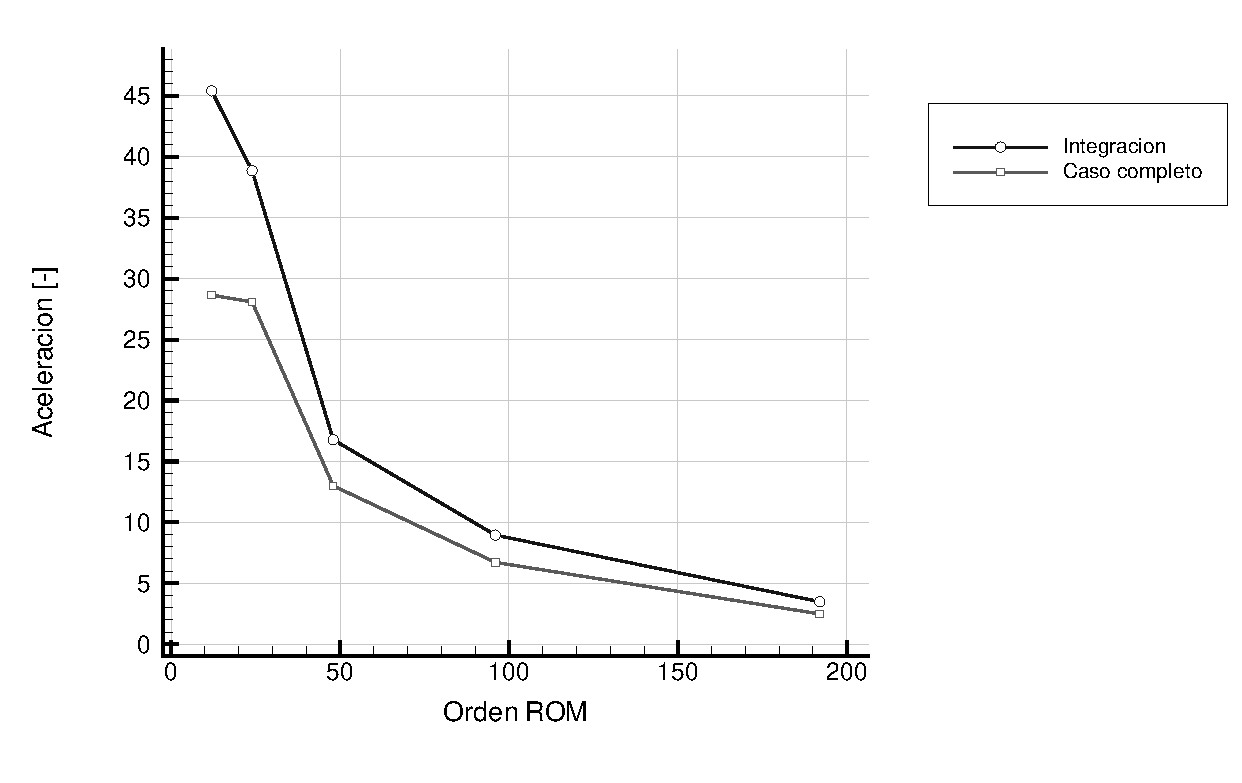
\includegraphics[width=\linewidth]{figures/tecplot/rom_aceleracion.pdf}\end{minipage}
\caption{Precisión y eficiencia de los ROM estacionarios: (a) máximo error de historia de cada salida y (b) aceleración de integración y de un caso incluyendo base y proyección. Los símbolos distinguen curvas en escala de grises.}\label{fig:romcoste}\end{figure}
\begin{figure}[htbp]\centering
\begin{minipage}{0.96\linewidth}\centering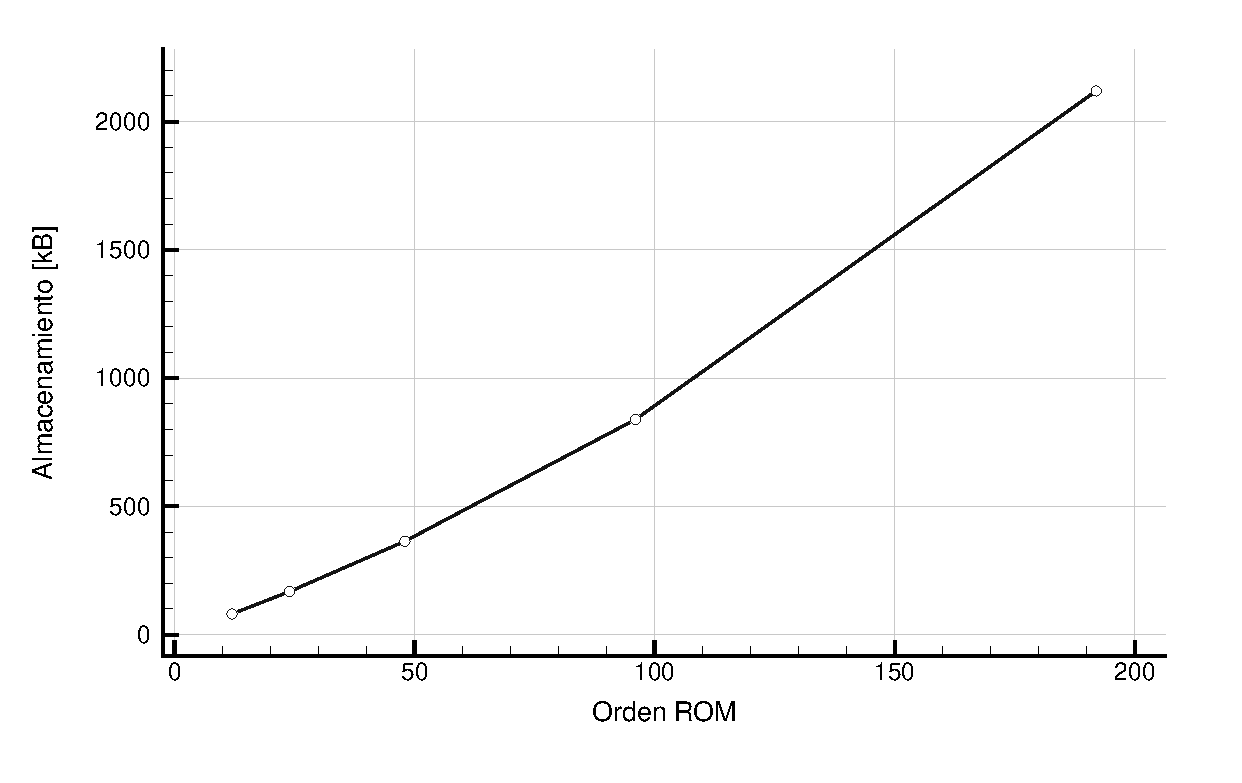
\includegraphics[width=\linewidth]{figures/tecplot/rom_operatorAndBasisBytes.pdf}\end{minipage}
\par\medskip
\begin{minipage}{0.96\linewidth}\centering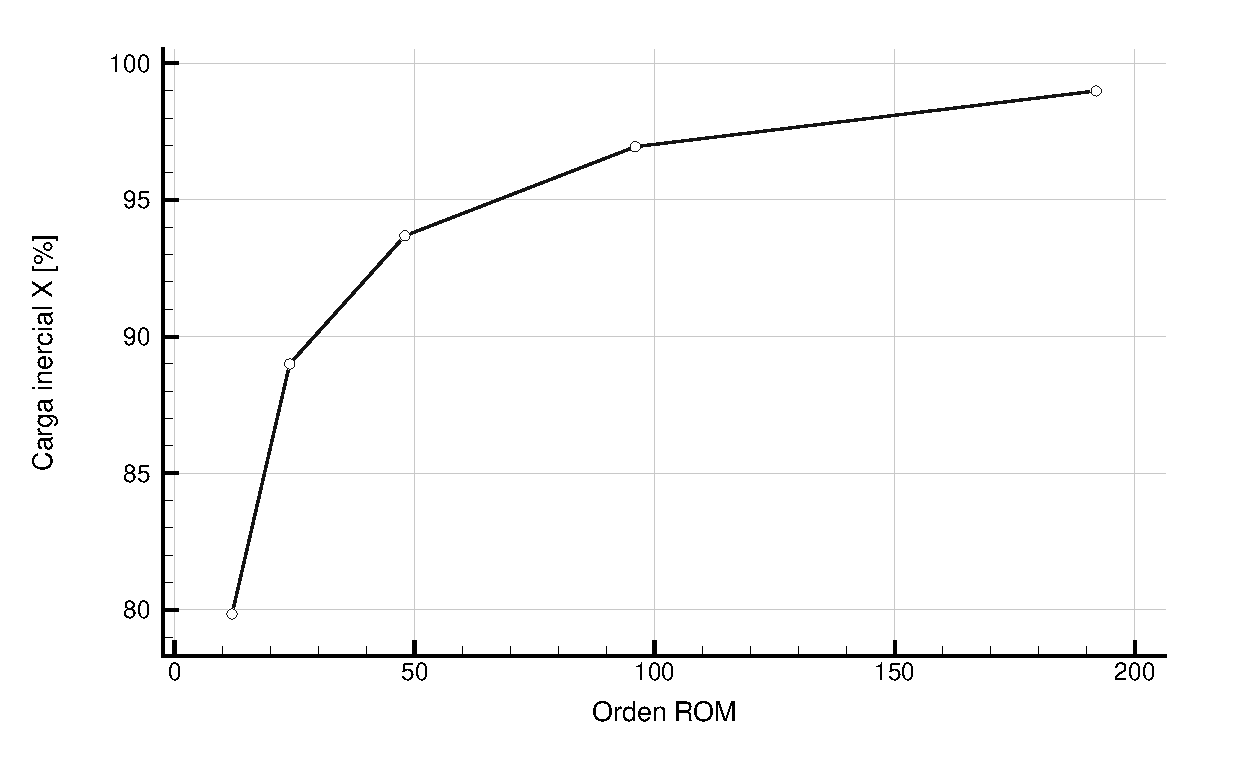
\includegraphics[width=\linewidth]{figures/tecplot/rom_massParticipationXPercent.pdf}\end{minipage}
\caption{Costo y participación de los ROM estacionarios: (a) almacenamiento de operadores y base y (b) participación de la carga inercial global X. Se conservan los datos históricos y sus definiciones; el almacenamiento no es memoria pico.}\label{fig:romcoste-continuacion}\end{figure}

El error de truncamiento se mide con la misma malla temporal en ambos modelos. Al comparar el MHT a pasos de 0.0025 y 0.00125 s, las diferencias de historia varían entre 0.0164 y 0.2051\%, con el máximo en la reacción basal. El error ROM192 de 0.0866\% no implica entonces una exactitud total inferior a 0.1\% respecto del problema continuo. Los errores de pico de todos los ROM y las diferencias temporales por salida se reúnen en el Apéndice~\ref{ap:datos}, de modo que la interpretación no dependa de una sola métrica.

\section{DISCUSIÓN}
\label{sec:discusion}
Los resultados permiten distinguir tres decisiones de modelado. La primera es cinemática: el elemento y las restricciones deben conservar los movimientos rígidos sin introducir resortes de penalización que contaminen el espectro. La segunda es rotodinámica: giroscopía, centrifugación y transporte derivan de una misma aproximación energética y deben transformarse conjuntamente. La tercera es de reducción: el número de modos se determina por las salidas y el contenido de la carga, no solo por la coincidencia de frecuencias bajas.

La comparación de teorías muestra que la precisión espacial no elimina el error de hipótesis. Para el voladizo menos esbelto, las discrepancias Euler--Bernoulli--Timoshenko alcanzan 21.21\% en el cuarto modo, aunque ambas discretizaciones converjan. En el MHT, retirar únicamente el cortante altera las bajas frecuencias entre aproximadamente 0.5 y 3.1\% sin cambiar sustancialmente las primeras once formas. Estos efectos son distintos de los producidos por el truncamiento modal, que conserva las hipótesis y matrices del modelo de referencia.

El análisis rotante conserva los términos de transporte que requiere el marco de ensamblaje. Una norma de Frobenius grande de un bloque no mide por sí sola su influencia sobre un modo, y mezclar bloques traslacionales y rotacionales añade una dependencia de unidades. Por ello, la interpretación física se apoya en equilibrio, ramas y respuestas recuperadas, no en atribuir dominancia modal únicamente a una norma matricial. Del mismo modo, un cruce de una rama con 1P o 3P identifica una coincidencia de frecuencias, no demuestra resonancia sin especificar la fuerza y su participación modal.

El barrido y la respuesta sísmica operativa corresponden a operadores congelados en un azimut. La MBC conserva las derivadas del cambio de coordenadas, pero no convierte automáticamente el sistema físico en invariante durante toda una revolución. Las raíces extraídas de \eqref{eq:qep} caracterizan ese sistema congelado; no establecen estabilidad de Floquet ni cubren raíces que no se calcularon. La recuperación con \eqref{eq:recuperacion} es consistente localmente con los mapas del instante de referencia, no una integración de la trayectoria nominal completa.

La comparación ROM se limita al estado detenido y sin precarga. Extender sus órdenes y ganancias al rotor en operación requiere actualizar la base y repetir la comparación bajo los operadores y fuerzas correspondientes. Tampoco se cuantifica aquí la diferencia frente a una simulación independiente de vigas geométricamente exactas, cascarones o sólidos. Los antecedentes de co-simulación \citep{maza2014,turello2023} proporcionan un marco para esa comparación, pero no constituyen resultados del presente cálculo.

Finalmente, la base fija, las inercias nominales, los centros de masa supuestos y los coeficientes de tren y amortiguamiento delimitan el significado de las respuestas. La formulación de viento y base flexible admite extensiones, pero las campañas estructurales de la Tabla~\ref{tab:campanas} no caracterizan la interacción aeroelástica o geotécnica de una instalación específica. El aporte cuantificado es la consistencia y eficiencia de un modelo estructural definido; su validación física requiere datos de carga, parámetros identificados y una referencia independiente.

\section{CONCLUSIONES}
La representación híbrida conserva los seis movimientos rígidos del elemento y del ensamblaje libre conectado. Su identificación se sustenta en cinemática, rango--nulidad y residuos normalizados; las frecuencias crudas cercanas a cero dependen de la escala espectral y no de un umbral decimal universal. Con base fija, el MHT tiene 804 coordenadas y un espectro elástico sin esos mecanismos.

La malla de 133 elementos difiere menos de 0.00935\% de la referencia refinada en sus primeras doce frecuencias estacionarias. Esa precisión no elimina el efecto de la teoría de viga: el cortante y la inercia rotacional cobran importancia al aumentar el orden modal o disminuir la esbeltez.

La derivación energética determina conjuntamente el bloque giroscópico, la fuerza centrífuga y su tangente. Su acoplamiento al resto de la estructura requiere conservar transporte inercial, derivada de masa y restricciones temporales. Los resultados operativos actualizados son consecuencia de esa cadena completa, y no de una sustitución aislada del momento angular del cubo.

En la comparación estacionaria, ROM48 reproduce las siete salidas de movimiento con error de historia inferior a 1\%, pero conserva 7.12\% en el momento basal. ROM192 reduce el máximo de las ocho salidas a 0.0866\%. La reacción requiere una base más amplia porque combina contribuciones que pueden ser poco visibles en un desplazamiento puntual.

El criterio de precisión modifica la ganancia computacional: la aceleración de integración pasa de 16.78 para ROM48 a 3.49 para ROM192; al incluir base y proyección, pasa de 13.00 a 2.49. La reducción es eficiente para las salidas y condiciones estudiadas, aunque el almacenamiento del ROM de mayor orden supera al del sistema disperso completo. Estas conclusiones apoyan una selección de fidelidad basada en la respuesta de interés, sin extrapolarla a estabilidad periódica, interacción aeroelástica calibrada o comportamiento local no modelado.

\appendix
% Restored from the existing formulation article and persisted evidence.
\section{Operadores elementales}\label{ap:elemento}

El orden elemental es $\bm q_e^\ell=[(\bm q_I^\ell)^\tr,(\bm q_J^\ell)^\tr]^\tr$, donde $\bm q_i^\ell=[u_i,v_i,w_i,\theta_{xi},\theta_{yi},\theta_{zi}]^\tr$. La extensión, en índices $(1,7)$, y la torsión, en $(4,10)$, utilizan
\begin{equation}
\bm K_{\rm ax}=\frac{EA}{L}\begin{bmatrix}1&-1\\-1&1\end{bmatrix},\qquad
\bm K_{\rm tor}=\frac{GJ_t}{L}\begin{bmatrix}1&-1\\-1&1\end{bmatrix}.
\end{equation}
Para cada plano se definen
\begin{align}
\phi&=\frac{12EI}{GA_sL^2},&a&=\frac{12EI}{L^3(1+\phi)},\nonumber\\
b&=\frac{6EI}{L^2(1+\phi)},&c&=\frac{(4+\phi)EI}{L(1+\phi)},\nonumber\\
d&=\frac{(2-\phi)EI}{L(1+\phi)}.
\end{align}
El bloque de flexión es
\begin{equation}
\bm K_{\rm fl}=\begin{bmatrix}
a&rb&-a&rb\\rb&c&-rb&d\\-a&-rb&a&-rb\\rb&d&-rb&c
\end{bmatrix}.
\end{equation}
Se emplean $(EI_z,GA_{sy},r=1)$ en índices $(2,6,8,12)$ y $(EI_y,GA_{sz},r=-1)$ en $(3,5,9,11)$. Insertar los cuatro bloques determina todas las entradas de $\bm K_e^\ell$.

Para $s=x/L$ y $\bm p=[1,s,s^2,s^3]$, la interpolación de un plano es $v=\bm p\bm C_v\bm d_y$, $\theta_z=\bm p\bm C_r\bm d_y$, con $\bm d_y=[v_I,\theta_{zI},v_J,\theta_{zJ}]^\tr$ y
\begin{equation}
\bm C_v=\frac1{1+\phi}\begin{bmatrix}
1+\phi&0&0&0\\
-\phi&L(1+\phi/2)&\phi&-L\phi/2\\
-3&-L(2+\phi/2)&3&-L(1-\phi/2)\\
2&L&-2&L
\end{bmatrix},
\end{equation}
\begin{equation}
\bm C_r=\frac1{1+\phi}\begin{bmatrix}
0&1+\phi&0&0\\
-6/L&-(4+\phi)&6/L&-(2-\phi)\\
6/L&3&-6/L&3\\0&0&0&0
\end{bmatrix}.
\end{equation}
Para el otro plano se utilizan $\bm d_z=[w_I,\theta_{yI},w_J,\theta_{yJ}]^\tr$, $\bm S_z=\operatorname{diag}(1,-1,1,-1)$, $w=\bm p\bm C_v\bm S_z\bm d_z$ y $\theta_y=-\bm p\bm C_r\bm S_z\bm d_z$, con el $\phi$ correspondiente. Los campos $u,\theta_x$ se interpolan linealmente. Estas relaciones definen $\bm N$; sus derivadas y los términos de cortante definen $\bm B$.

Para propiedades constantes, cuatro puntos de Gauss integran exactamente los productos de grado máximo seis de masa y giroscopía. La fuerza y la tangente centrífugas se evalúan con la misma interpolación y cuadratura. La rigidez anterior es cerrada, no obtenida mediante integración reducida. Una formulación de secciones acopladas requiere construir y discretizar su energía general; no se obtiene insertando acoplamientos arbitrarios en estos cuatro bloques.


\section{Matrices energéticas del giro}\label{ap:gyro}

\subsection{Cinemática exacta del movimiento nominal}
Sea $\bm R_0(t)$ la rotación nominal y $\bm W=\Sx{\Omega}$, con $\dot{\bm R}_0=\bm R_0\bm W$. El vector $\bm\Omega=\Omega\bm e_\Omega$ tiene dirección fija. Se elige $\bm R_0(0)=\I$, de modo que $\bm R_0\bm W\bm R_0^\tr=\bm W$: sus componentes nominales e inerciales coinciden para este giro. Para una sección, $\bm a$ localiza la línea de referencia respecto al origen del rotor, y $\bm r$ localiza su centro de masa. En este apartado se escribe $m=\mu$, $\bm J=\bm j_C$ para cantidades por longitud; las mismas expresiones describen un cuerpo concentrado al utilizar su masa y su tensor.

La perturbación rotacional se representa mediante $\bm E=\exp(\Sx{\theta})$. La posición inercial del centro de masa y su tensor en componentes nominales son, respectivamente,
\begin{equation}
\bm x_C=\bm R_0(\bm a+\bm u+\bm E\bm r),\qquad
\bm J_C^{(n)}(\bm\theta)=\bm E\bm J\bm E^\tr.
\end{equation}
El origen nominal se considera fijo; su excitación traslacional se incorpora después mediante el movimiento de base. Con el Jacobiano izquierdo $\bm J_\ell(\bm\theta)$ del grupo de rotaciones,
\begin{align}
\bm v_C&=\bm W(\bm a+\bm u+\bm E\bm r)+\dot{\bm u}
+\Sx{J_\ell(\bm\theta)\dot{\bm\theta}}\bm E\bm r,\nonumber\\
\bm\omega&=\bm\Omega+\bm J_\ell(\bm\theta)\dot{\bm\theta}.
\label{apx:eq:exactvelocity}
\end{align}
Las velocidades están expresadas en componentes nominales. La energía que genera todos los términos inerciales es
\begin{equation}
\mathcal T=\tfrac12m\bm v_C^\tr\bm v_C
+\tfrac12\bm\omega^\tr\bm E\bm J\bm E^\tr\bm\omega.
\label{apx:eq:exactT}
\end{equation}

\subsection{Expansión de segundo orden}
Se retienen términos hasta grado dos en $\bm\eta=[\bm u^\tr,\bm\theta^\tr]^\tr$ y $\dot{\bm\eta}$. Las expansiones necesarias son
\begin{align}
\bm E&=\I+\Sx{\theta}+\tfrac12\Sx{\theta}^2+\mathcal O(3),\nonumber\\
\bm J_\ell\dot{\bm\theta}&=\dot{\bm\theta}
+\tfrac12\bm\theta\times\dot{\bm\theta}+\mathcal O(3).
\end{align}
Así, la parte cuadrática adopta la forma de \citet{meirovitch1997},
\begin{equation}
\mathcal T^{(2)}=\tfrac12\dot{\bm\eta}^\tr\bm M_6\dot{\bm\eta}
+\dot{\bm\eta}^\tr\bm A_6\bm\eta
+\tfrac12\bm\eta^\tr\bm H_\Omega\bm\eta.
\label{apx:eq:T2}
\end{equation}
Para expresar sus coeficientes se definen
\begin{align}
\bm B&=[\I,-\Sx{r}],&\bm E_\theta&=[\bm0,\I],\nonumber\\
\bm b&=\bm a+\bm r,&\bm h&=\bm J\bm\Omega,\nonumber\\
\bm v_0&=\bm W\bm b,&\bm a_0&=\bm W^2\bm b,
\end{align}
y la matriz simétrica
\begin{equation}
\mathcal H(\bm a,\bm b)=\tfrac12(\bm a\bm b^\tr+\bm b\bm a^\tr)
-(\bm a^\tr\bm b)\I.
\end{equation}
Esta satisface $\bm a^\tr\Sx{\theta}^2\bm b=\bm\theta^\tr\mathcal H(\bm a,\bm b)\bm\theta$. Los coeficientes de la ec.~\eqref{eq:energia2} quedan determinados por
\begin{align}
\bm M_6&=m\bm B^\tr\bm B+\bm E_\theta^\tr\bm J\bm E_\theta,\label{apx:eq:M6}\\
\bm A_6&=m\bm B^\tr\bm W\bm B+\bm E_\theta^\tr\bm A_\theta\bm E_\theta,\nonumber\\
\bm A_\theta&=\bm J\bm W-\tfrac12\Sx{h}+m\mathcal H(\bm v_0,\bm r).
\label{apx:eq:A6}
\end{align}
La masa coincide con la ec.~\eqref{eq:masa6}. El último término de $\bm A_\theta$ es simétrico y, con coeficientes nominales constantes, contribuye solamente mediante una derivada temporal total. Se mantiene para explicitar la expansión, aunque desaparece del operador giroscópico.

\subsection{Matriz giroscópica completa}
Al aplicar las ecuaciones de Lagrange a la ec.~\eqref{eq:energia2}, el término de velocidad resulta de la parte antisimétrica de $\bm A_6$:
\begin{align}
\bm G_{c,6}&=\bm A_6-\bm A_6^\tr\nonumber\\
&=2m\bm B^\tr\bm W\bm B+\bm E_\theta^\tr\bm G_\theta\bm E_\theta,\label{apx:eq:G6}\\
\bm G_\theta&=\bm J\bm W+\bm W\bm J-\Sx{J\Omega}.
\label{apx:eq:Gtheta}
\end{align}
El subíndice $c$ indica componentes corrotantes. Para mostrar el acoplamiento entre traslaciones y rotaciones, se escribe
\begin{equation}
\bm G_{c,6}=\begin{bmatrix}
2m\bm W&-2m\bm W\Sx{r}\\
2m\Sx{r}\bm W&\bm G_\theta-2m\Sx{r}\bm W\Sx{r}
\end{bmatrix}.
\label{apx:eq:Gblocks}
\end{equation}
Por construcción, $\bm G_{c,6}^\tr=-\bm G_{c,6}$ y $\dot{\bm\eta}^\tr\bm G_{c,6}\dot{\bm\eta}=0$: el operador no disipa energía. Esta propiedad corresponde a la giroscopía, no necesariamente a la matriz completa que multiplica velocidades después de transformar las coordenadas.

Para giro alrededor de un eje principal, $\bm\Omega=\Omega\bm e_1$ y $\bm J=\operatorname{diag}(J_1,J_2,J_3)$, el coeficiente del acoplamiento angular en el plano $2$--$3$ es $(J_2+J_3-J_1)\Omega$. El término aislado $\Sx{J\Omega}$ no reproduce la ec.~\eqref{apx:eq:Gtheta} en coordenadas corrotantes. Su aparición con otro signo en un marco inercial, deducida más adelante, no constituye una formulación alternativa: responde al transporte de la misma ecuación.

\subsection{Potencial centrífugo y equilibrio mantenido}
Dentro de la expansión de segundo orden, la parte que depende de posición define simultáneamente la carga centrífuga y su tangente. Con fuerzas centrífugas en el segundo miembro,
\begin{align}
\bm f_{\Omega,0}&=-m\bm B^\tr\bm a_0-\bm E_\theta^\tr(\bm\Omega\times\bm h),\nonumber\\
\bm f_\Omega(\bm\eta)&=\bm f_{\Omega,0}-\bm K_{\Omega,c}\bm\eta,\label{apx:eq:fOmega}\\
\bm K_{\Omega,c}&=m\bm B^\tr\bm W^2\bm B+\bm E_\theta^\tr\bm K_\theta\bm E_\theta,\nonumber\\
\bm K_\theta&=m\mathcal H(\bm a_0,\bm r)+\bm W\bm J\bm W
-\mathcal H(\bm h,\bm\Omega).
\label{apx:eq:KOmega}
\end{align}
En consecuencia, $\bm H_\Omega=-\bm K_{\Omega,c}$. Este operador no sustituye a la rigidez geométrica inducida por las tensiones de equilibrio.

Si $\bm h$ y $\bm\Omega$ no son paralelos, el movimiento uniforme requiere un par de mantenimiento $\bm\tau_0=\bm\Omega\times\bm h$. Este par equilibra el término angular nominal de la ec.~\eqref{apx:eq:fOmega}. En la turbina completa puede transmitirse a través del tren y sus restricciones; no se añade una segunda carga cuando esa transmisión ya está representada. Su tangente depende de la ley de carga: un par de componentes constantes en el cuerpo perturbado y uno constante en el marco nominal producen, respectivamente, $+\tfrac12\Sx{\tau_0}$ y $-\tfrac12\Sx{\tau_0}$ en el residual linealizado. Una ley elástica o de control requiere su propia derivada.

Los operadores elementales se obtienen mediante la misma interpolación $\bm N$ utilizada por la masa:
\begin{align}
\bm G_{c,e}&=\int_0^L\bm N^\tr\bm G_{c,6}\bm N\,\dd x,\nonumber\\
\bm K_{\Omega,c,e}&=\int_0^L\bm N^\tr\bm K_{\Omega,c}\bm N\,\dd x,\nonumber\\
\bm f_{\Omega,0,e}&=\int_0^L\bm N^\tr\bm f_{\Omega,0}\,\dd x.
\end{align}
Se conserva la dependencia espacial de $\bm a(x)$; no se aplica una aceleración centrífuga uniforme a toda la pala. Al ensamblar, se denominan $\bm F_{\Omega,0}$ y $\bm K_{\Omega,c}^{f}$ a la fuerza y la tangente nodales completas. En ese nivel, $\bm F_\Omega(\bm q)=\bm F_{\Omega,0}-\bm K_{\Omega,c}^{f}\bm q$, sin confundirlas con las cantidades seccionales por longitud.


\section{Mapas temporales y transformación multiblade}\label{ap:mapas}

Para tres palas equiespaciadas con correspondencia biyectiva de coordenadas homólogas, se construye $\bm H(t)$ con bloques $\operatorname{blkdiag}(\bm Q_b,\bm Q_b)$, donde $\bm Q_b=\bm R_0\bm Q_{b0}$. Se excluyen las raíces ya condensadas al cubo. Los bloques estacionarios son identidades. Para cada coordenada homóloga, la transformación colectiva--coseno--seno de \citet{bir2008} es
\begin{equation}
\bm B_3=\begin{bmatrix}
1&\cos\psi_1&\sin\psi_1\\
1&\cos\psi_2&\sin\psi_2\\
1&\cos\psi_3&\sin\psi_3
\end{bmatrix},\qquad
\psi_b=\psi+\frac{2\pi(b-1)}3.
\end{equation}
Al agrupar las coordenadas primero por pala se utiliza $\bm B_3\otimes\I$ y se conserva la identidad en las partes estacionarias. Con $\bm B_{\rm mbc}$ como matriz ampliada,
\begin{align}
\bm P_{\rm mbc}&=\bm H\bm B_{\rm mbc},\nonumber\\
\dot{\bm P}_{\rm mbc}&=\dot{\bm H}\bm B_{\rm mbc}+\bm H\dot{\bm B}_{\rm mbc},\nonumber\\
\ddot{\bm P}_{\rm mbc}&=\ddot{\bm H}\bm B_{\rm mbc}
+2\dot{\bm H}\dot{\bm B}_{\rm mbc}+\bm H\ddot{\bm B}_{\rm mbc}.
\end{align}
Al introducir $\bm z=\bm P_{\rm mbc}\bm y$, los operadores $\overline{\bm M},\overline{\bm D},\overline{\bm K}$ se obtienen aplicando nuevamente la ec.~\eqref{eq:mpc}, con $\bm T$ sustituida por $\bm P_{\rm mbc}$ y operadores de entrada $\bm M_r,\bm D_r,\bm K_r$. El Apéndice C presenta la inversa y las derivadas explícitas. La giroscopía física y las derivadas multiblade pertenecen a etapas diferentes de una misma transformación; conservar ambas no implica duplicar fuerzas.


La derivada de la masa después de las restricciones es
\begin{align}
\dot{\bm M}_r={}&\dot{\bm T}^\tr\bm M\bm T+\bm T^\tr\dot{\bm M}\bm T
+\bm T^\tr\bm M\dot{\bm T}.
\end{align}
Esta identidad permite separar nuevamente la derivada de masa de la parte antisimétrica del operador inercial de velocidad.

La inversa multiblade y sus derivadas son
\begin{equation}
\bm B_3^{-1}=\frac13\begin{bmatrix}
1&1&1\\2\cos\psi_1&2\cos\psi_2&2\cos\psi_3\\
2\sin\psi_1&2\sin\psi_2&2\sin\psi_3
\end{bmatrix},
\end{equation}
\begin{align}
[\dot{\bm B}_3]_{b,:}&=\Omega[0,-\sin\psi_b,\cos\psi_b],\nonumber\\
[\ddot{\bm B}_3]_{b,:}&=-\Omega^2[0,\cos\psi_b,\sin\psi_b].
\end{align}
Para los bloques de pala, $\dot{\bm H}=\bm W_H\bm H$ y $\ddot{\bm H}=\bm W_H^2\bm H$, con $\bm W_H$ nula en las coordenadas estacionarias. Estas derivadas no desaparecen al seleccionar un azimut para evaluar los operadores.

Para completar el paso temporal de aceleración media, se define
\begin{align}
\bm K_{\rm eff}&=\bm K_r+\frac4{\Delta t^2}\bm M_r+\frac2{\Delta t}\bm D_r,\nonumber\\
\bm f_{\rm eff}&=\bm f_{n+1}
+\bm M_r\left(\frac4{\Delta t^2}\bm z_n+\frac4{\Delta t}\dot{\bm z}_n+\ddot{\bm z}_n\right)\nonumber\\
&\quad+\bm D_r\left(\frac2{\Delta t}\bm z_n+\dot{\bm z}_n\right),\nonumber\\
\bm K_{\rm eff}\bm z_{n+1}&=\bm f_{\rm eff}.
\end{align}
Las velocidades y aceleraciones se recuperan de las relaciones de Newmark. El mismo esquema puede aplicarse a operadores reducidos, manteniendo coherentes carga, coordenadas y recuperación física \citep{newmark1971}.


\section{Integración y recuperación}\label{ap:solucion}

Se presenta la integración en las coordenadas independientes $\bm z$, anteriores a multiblade. En el análisis local, $\bm M_r,\bm D_r,\bm K_r$ se congelan en el mismo estado operativo. El método de aceleración media de Newmark se define mediante
\begin{align}
\bm z_{n+1}&=\bm z_n+\Delta t\dot{\bm z}_n
+\tfrac{\Delta t^2}{4}(\ddot{\bm z}_n+\ddot{\bm z}_{n+1}),\nonumber\\
\dot{\bm z}_{n+1}&=\dot{\bm z}_n+\tfrac{\Delta t}{2}
(\ddot{\bm z}_n+\ddot{\bm z}_{n+1}).
\end{align}
La matriz efectiva es $\bm K_r+4\bm M_r/\Delta t^2+2\bm D_r/\Delta t$; se conserva completa, aunque sea no simétrica. El Apéndice C presenta el segundo miembro. Las propiedades del integrador no eliminan una inestabilidad física de los operadores.

Para $\delta\bm q=\bm T(t)\bm z$, la recuperación requiere
\begin{align}
\delta\dot{\bm q}&=\bm T\dot{\bm z}+\dot{\bm T}\bm z,\nonumber\\
\delta\ddot{\bm q}&=\bm T\ddot{\bm z}+2\dot{\bm T}\dot{\bm z}+\ddot{\bm T}\bm z.
\end{align}
Se añade $\bm\Gamma_f\bm a_g$ para recuperar la aceleración absoluta de perturbación; la aceleración centrípeta nominal debe añadirse por separado si se requiere la aceleración total. Cuando se congelan los operadores, también se evalúan el mapa y sus derivadas en el azimut de referencia: se obtiene una reconstrucción local, no una trayectoria periódica completa.

Las reacciones se recuperan del residual completo del sistema físico, antes de eliminar apoyos y restricciones. Su proyección sobre coordenadas admisibles es nula. Las resultantes incrementales seccionales se obtienen como $\delta\bm n=\bm K_s\bm B\bm T_e\delta\bm q_e$; para la demanda total se suman las resultantes del equilibrio.


\section{Fuentes, unidades y trazabilidad}\label{ap:datos}
La geometría conserva 138 nodos y 133 elementos de viga. Se eliminan de esta visualización únicamente los cuatro elementos heredados de penalización tipo 3, sustituidos en el modelo vigente por restricciones exactas. Las coordenadas se expresan en metros y cada nodo conserva el orden $[u_x,u_y,u_z,\theta_x,\theta_y,\theta_z]$.

Los resultados operativos proceden de las campañas corregidas de septiembre y se extraen del archivo de evidencia de este manuscrito. Las comparaciones ROM y de refinamiento son estacionarias e históricas. La biblioteca Tecplot conserva la relación por figura entre fuentes, unidades, configuración, dataset, macro, layout y paquete nativo. No se lanzaron campañas para completar las figuras.

Las envolventes de la turbina tienen una finalidad ilustrativa. La formulación y la malla computacional siguen siendo de vigas; las superficies no incorporan rigideces, masas ni grados de libertad de sólidos. Para las formas complejas de la biblioteca se conservan ramas individuales, fases de $0^\circ$ y $90^\circ$, normalización por la máxima traslación nodal compleja y amplificación declarada. No se construye una forma modal a partir de la frecuencia media de un grupo.


\begin{thebibliography}{99}
\bibitem[Bir(2008)]{bir2008} Bir, G.S. \emph{Multiblade Coordinate Transformation and Its Application to Wind Turbine Analysis}. NREL/CP-500-42553, 2008. \url{https://www.nrel.gov/docs/fy08osti/42553.pdf}.
\bibitem[Griffith(2013)]{griffith2013} Griffith, D.T. \emph{The SNL100-01 Blade: Carbon Design Studies for the Sandia 100-meter Blade}. Sandia National Laboratories, SAND2013-1178, 2013. \doi{10.2172/1093695}.
\bibitem[Maza et al.(2014)]{maza2014} Maza, M.S., Preidikman, S. y Flores, F.G. Unsteady and non-linear aeroelastic analysis of large horizontal-axis wind turbines. \emph{International Journal of Hydrogen Energy}, 39(16):8813--8820, 2014. \doi{10.1016/j.ijhydene.2013.12.028}.
\bibitem[Meirovitch(1997)]{meirovitch1997} Meirovitch, L. \emph{Principles and Techniques of Vibrations}. Prentice Hall, 1997. Secciones 4.4, 4.7 y 7.17.
\bibitem[Newmark y Rosenblueth(1971)]{newmark1971} Newmark, N.M. y Rosenblueth, E. \emph{Fundamentals of Earthquake Engineering}. Prentice Hall, 1971.
\bibitem[Reddy(2006)]{reddy2006} Reddy, J.N. \emph{An Introduction to the Finite Element Method}. 3.\textsuperscript{a} edición, McGraw-Hill, 2006.
\bibitem[Simo(1985)]{simo1985} Simo, J.C. A finite strain beam formulation. The three-dimensional dynamic problem. Part I. \emph{Computer Methods in Applied Mechanics and Engineering}, 49(1):55--70, 1985. \doi{10.1016/0045-7825(85)90050-7}.
\bibitem[Turello et al.(2023)]{turello2023} Turello, D.F., Maza, M.S., Preidikman, S., Flores, F.G. y Pinto, F. Interacción suelo-estructura no-lineal en el modelado de torres eólicas de eje horizontal ante carga sísmica. \emph{Mecánica Computacional}, XL:639--650, 2023. \url{https://amcaonline.org.ar/ojs/index.php/mc/article/view/6595}.
\end{thebibliography}
\end{document}
